\chapter{METHODOLOGY}

This chapter introduces the research design and evaluation strategy and then describes the system design decisions underlying each component. Chapter~4 contains detailed implementation evidence and experimental results, and Chapter~5 contains quantitative model evaluation.
% ─────────────────────────────────────────────────────────────
\section{Research Design and Evaluation Strategy}
\label{sec:research_design}

This project follows a \textbf{Design Science Research (DSR)} methodology, a well-established paradigm for thesis work with an engineering focus, in which the main artefact is a designed system evaluated against defined utility criteria~\cite{Hevner2004}. DSR is appropriate because the contribution is a working system, not an algorithm or theory. The research process consists of three phases:

\begin{enumerate}
\item \textbf{Requirements and Design}. (Section~\ref{sec:user_req}) Functional requirements are drawn from the elderly-care context and, together with the gaps identified in Chapter~2, shape the design of the hardware, system architecture, ML pipeline, and AI assistant. \item \textbf{Implementation.}  The artefact (hardware node, Flask backend, web dashboard and Flutter mobile app) is built to meet the functional requirements and validated through system-level experiments in Chapter~\ref{chap:experiments}. \item \textbf{Evaluation.} For RQ1, end-to-end functional tests and latency benchmarking are conducted (Section~\ref{sec:performance}). For RQ2, the precision, recall, F1-score and false positive rate of the Isolation Forest algorithm are evaluated (Section~\ref{sec:ml_validation}). For RQ3, Rule mode commands are tested manually and LLM and Gemini interactions are evaluated qualitatively (Section~\ref{sec:rq_answers}).


\end{enumerate}

An important limitation of this research design is the lack of an independent usability study with elderly or caregiver participants. The developer walkthrough in Section~\ref{sec:usability} is a consistency check within the team, not a usability evaluation. This is explicitly stated in the limitations (see Section~\ref{sec:limitations_conclusion}).

% ─────────────────────────────────────────────────────────────
\section{User Requirement Analysis}
\label{sec:user_req}

Functional requirements were identified based on the problem context and target users (elderly residents and family caregivers):

\begin{enumerate}
    \item \textbf{Environmental monitoring}: the system shall continuously collect temperature, humidity, ambient light and motion data from sensor nodes inside the home and provide these readings to caregivers in real time.
   \item \textbf{Physiological monitoring}: the system should be able to receive heart-rate data from a BLE wearable device and store individual readings for trend monitoring and anomaly detection.
    \item \textbf{Anomaly detection and alerting}: the system shall automatically detect abnormal heart-rate patterns using a machine learning model and emit real-time alerts to all connected caregiver interfaces.
    \item \textbf{Remote device control}: caregivers should be able to turn on or off relay connected devices (lights, fans) from the web dashboard and the mobile application.
    \item \textbf{Floor-plan visualisation}: the system shall provide an
    interactive floor-plan editor that allows caregivers to define room boundaries
    and assign sensor/actuator devices to specific rooms.
    \item \textbf{Care and schedule management}: the system shall provide a calendar interface to manage daily activities, medical appointments, and notes and to create recurring medicine reminders. Real-time notifications will be sent to web and mobile interfaces.
    \item \textbf{Conversational AI assistant}: the system shall provide natural-language interaction for device control, status inquiries, and health information through a context-aware AI assistant (Alfred) accessible from both interfaces. Alfred will also detect distress phrases in the chat (e.g. \textit{``cứu tôi''}, \textit{``chest pain''}, \textit{``SOS''}) and automatically trigger an emergency alert and caregiver email.
    \item \textbf{User authentication and role management}: The system shall provide support for user authentication and enable role separation for caregivers and administrators.
\end{enumerate}

Figure~\ref{fig:usecase_diagram} maps these requirements as a UML use case
diagram. There are four actors: the \textit{User} (caregiver), the
\textit{Admin}, the \textit{ESP32 Sensor Node}, and the \textit{Coospo H6}
BLE monitor. The 26 use cases are grouped into nine feature packages.
The Admin actor inherits all User interactions via a generalisation arrow
and additionally has access to a separate Admin-Only package covering
user management, alert rule configuration, alert statistics, and automation
rule management. The two hardware actors interact only through the
Monitoring \& Detection package, which handles sensor data ingestion and
anomaly detection.

\begin{figure}[p]
\centering
\makebox[\textwidth][c]{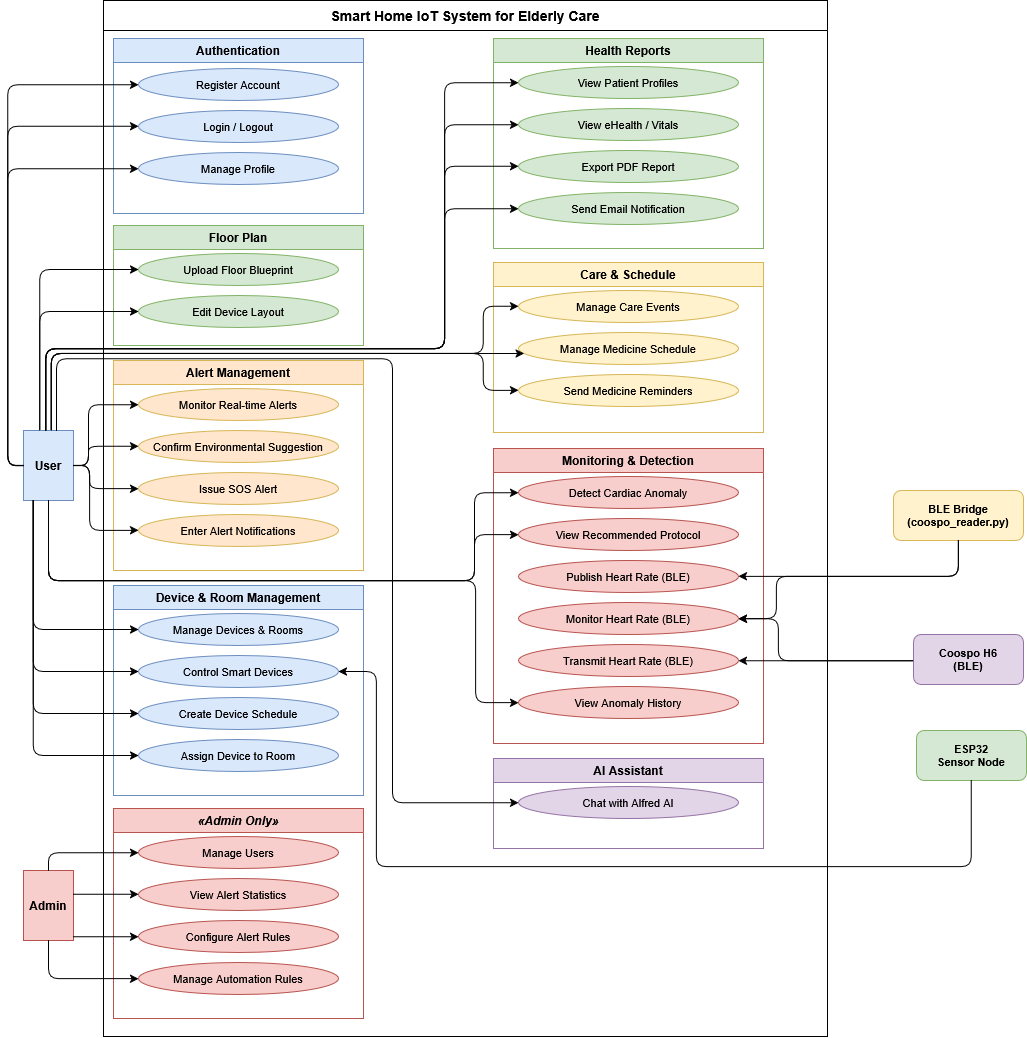
\includegraphics[width=\textwidth,height=0.92\textheight,keepaspectratio]{images/fig_usecase_diagram.png}}
\caption[UML use case diagram of the Smart Home IoT System for Elderly Care]{%
  UML use case diagram of the Smart Home IoT System for Elderly Care.
  Four actors interact with 26 use cases grouped into nine feature packages:
  \textit{User} (caregiver) accesses Authentication, Floor Plan, Alert Management,
  Device \& Room Management, Health Reports, Care \& Schedule, Monitoring \& Detection,
  and AI Assistant packages.
  \textit{Admin} inherits all User interactions via a generalisation arrow and additionally
  accesses the \textit{«Admin Only»} package (Manage Users, Configure Alert Rules,
  View Alert Statistics, Manage Automation Rules).
  \textit{ESP32 Sensor Node} and \textit{Coospo H6 (BLE)} are hardware actors that
  publish data through the Monitoring \& Detection package.}
\label{fig:usecase_diagram}
\end{figure}

% ─────────────────────────────────────────────────────────────
\section{Hardware Platform and Sensor Suite}
\label{sec:hardware_method}

\subsection{Microcontroller Selection}

The hardware node is based on the \textbf{ESP32-WROOM-32} module (Espressif Systems). The ESP32 integrates a dual-core Tensilica LX6 processor, clocked at up to 240\,MHz, along with 520\,KB of on-chip SRAM and 4\,MB of SPI Flash. Compared with the older ESP8266, the ESP32 integrates Wi-Fi (802.11\,b/g/n) and Bluetooth~4.2 (including BLE) into a single system-on-chip, making it well suited for IoT applications that require stable cloud communication while supporting nearby Bluetooth peripherals.

Key characteristics relevant to this design:

\begin{itemize}

\item \textbf{ADC}: two 12-bit SAR ADC units (18 ADC-capable channels across 34 GPIO pins);
here used to read the ambient-light LDR on GPIO 32 at 4096 discrete levels.
\item \textbf{Security engine}: hardware accelerators for AES, SHA-256,
RSA-2048, and ECC allow \texttt{WiFiClientSecure} to support TLS\,1.2
without an external cryptographic chip, enabling secure MQTT over
port~8883. On the Python backend side, the MQTT client uses
\texttt{ssl.create\_default\_context()} which verifies the broker
certificate against the system CA bundle; since EMQX Cloud provides a
certificate signed by a recognised CA, no manual CA file distribution
is required.
\item \textbf{Power}: 3.3\,V logic; an HLK-PM01 module on the PCB
converts 220\,V AC mains to a regulated 3.3\,V DC supply.
\item \textbf{Dual-core}: The ESP32 integrates two Tensilica LX6 cores.
In this firmware, all tasks (Wi-Fi keepalive, MQTT processing, sensor
acquisition, relay control, and LCD refresh) run sequentially inside the
single Arduino \texttt{loop()} on the default core, keeping the firmware
simple and avoiding inter-core synchronisation overhead.

\end{itemize}

\subsection{Sensor Suite and Actuators}

The node comprises four input sensors and two relay-based actuators.
Their key specifications are listed in Table~\ref{tab:sensor_specs}, and
the complete GPIO assignments are listed in Table~\ref{tab:pins}.

\begin{table}[H]
\centering
\caption{Sensor specifications for the ESP32 node}
\label{tab:sensor_specs}
\small
\begin{tabular}{p{3cm}p{3.5cm}p{4.5cm}p{2.5cm}}
\toprule
\textbf{Sensor} & \textbf{Interface} & \textbf{Range / Resolution} & \textbf{Notes} \\
\midrule
DHT11           & 1-Wire (GPIO\,15)    & 0--50\,$^\circ$C, $\pm2\,^\circ$C;\newline 20--80\% RH, $\pm5$\% & 5\,s publish interval \\
LDR             & ADC (GPIO\,32)       & 0--4095 raw, normalised 0--100 & 12-bit SAR ADC \\
PIR (HC-SR501)  & Digital (GPIO\,33)   & Binary: DETECTED / CLEAR       & Edge-triggered publish \\
Coospo H6       & BLE GATT\,0x2A37~\cite{BluetoothSIG2011}     & 30--240\,bpm, $\pm$1\,bpm      & Python BLE bridge \\
\bottomrule
\end{tabular}
\end{table}

\begin{table}[H]
\centering
\caption{ESP32 GPIO pin assignments}
\label{tab:pins}
\small
\begin{tabularx}{\textwidth}{@{}l c l X@{}}
\toprule
\textbf{Component} & \textbf{GPIO} & \textbf{Mode} & \textbf{Description} \\
\midrule
DHT11 & 15 & Digital input & Temperature \& humidity sensor (1-wire) \\
LDR (photoresistor) & 32 & ADC input & Ambient light, raw 0--4095, normalised 0--100 \\
PIR motion sensor & 33 & Digital input & Motion detection (edge-triggered) \\
Relay 1 (\texttt{den}) & 17 & Digital output & Light relay (active-high) \\
Relay 2 (\texttt{quat}) & 16 & Digital output & Fan relay (active-high)$^\dagger$ \\
I2C SDA (LCD) & 21 & I2C data & 16x2 LCD backpack data line \\
I2C SCL (LCD) & 22 & I2C clock & 16x2 LCD backpack clock line \\
Button 1 & 0 & Digital input & Physical toggle for Relay 1 \\
Button 2 & 2 & Digital input & Physical toggle for Relay 2$^\dagger$ \\
\bottomrule
\multicolumn{4}{@{}p{\textwidth}@{}}{\footnotesize $^\dagger$ P2 connector (Button~2 / Relay~2) damaged during testing; physical button non-functional but MQTT software control remains operational.} \\
\end{tabularx}
\end{table}

The DHT11 was selected over the more accurate DHT22 ($\pm0.5\,^\circ$C) and SHT31 ($\pm0.3\,^\circ$C) due to its lower cost and availability, making it suitable for a prototype. Its $\pm2\,^\circ$C tolerance is sufficient since temperature is used as \textit{contextual} input to the anomaly pipeline, not a clinical measurement (see Section~\ref{sec:future}).

Due to Wi-Fi/BLE coexistence constraints on the ESP32, the heart-rate acquisition from the \textbf{Coospo H6} chest strap (Figure~\ref{fig:coospo_h6}) is offloaded to a Python service that reads BPM via BLE GATT~\cite{BluetoothSIG2011} and forwards it at $\sim$1\,Hz to the MQTT topic \texttt{home/sensors/heart\_rate}. If disconnected, the service retries with a linear back-off ($\min(5 \times \mathit{retry},\,30)$\,s) and re-subscribes by MAC address. Gaps during outages are not buffered and appear as missing segments in the BPM chart, which is noted as a hardware limitation in Section~\ref{sec:future}.


\begin{figure}[H]
\centering

\includegraphics[width=0.50\textwidth]{images/coospo_h6.png}
\caption[Coospo H6 BLE heart-rate monitor]{Coospo H6 BLE chest-strap heart-rate monitor (GATT 0x2A37, $\sim$1\,Hz).}
\label{fig:coospo_h6}
\end{figure}

\subsection{Hardware Platform (PCB)}

The breadboard prototype was replaced by an ESP32 node on a two-layer PCB which contains the ESP32 module, relay driver circuits (2N3904 NPN transistors and 1N4007 flyback diodes), an HLK-PM01 AC/DC power supply, sensor connectors and touch-button inputs as a single assembly. This board is from previous hardware coursework and is reused in this thesis as the physical platform for the node. As such, the contribution of this thesis at the hardware layer is the firmware, sensor integration and BLE bridge, not the board design itself.
For completeness, Figure~\ref{fig:pcb_all} presents the schematic, the routed layout and 3D render of the board.

\begin{figure}[htbp]
  \centering
  \begin{subfigure}[b]{0.48\textwidth}
    \centering
    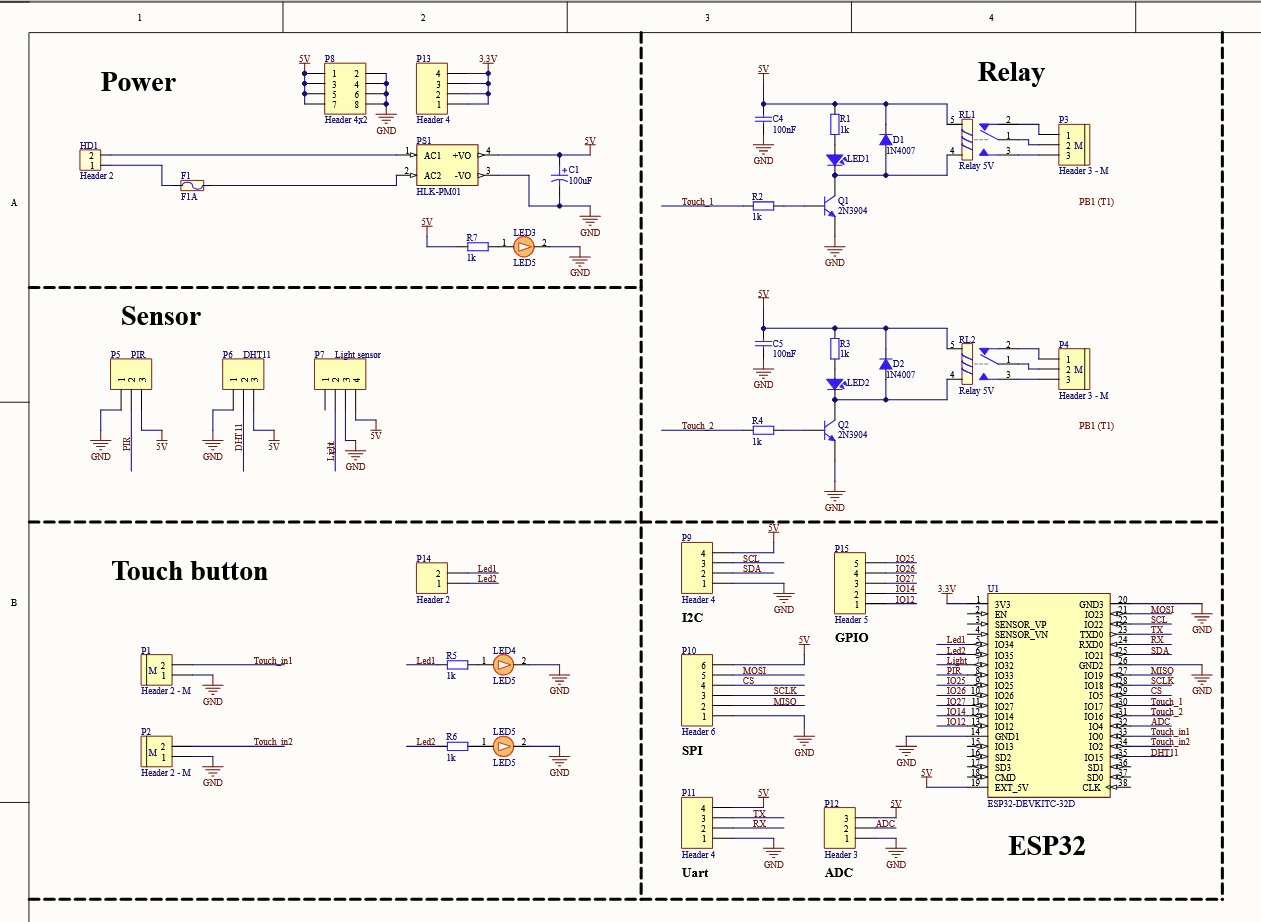
\includegraphics[width=\textwidth]{images/pcb_schematic.png}
    \caption{PCB schematic}
    \label{fig:pcb_schematic}
  \end{subfigure}
  \hfill
  \begin{subfigure}[b]{0.48\textwidth}
    \centering
    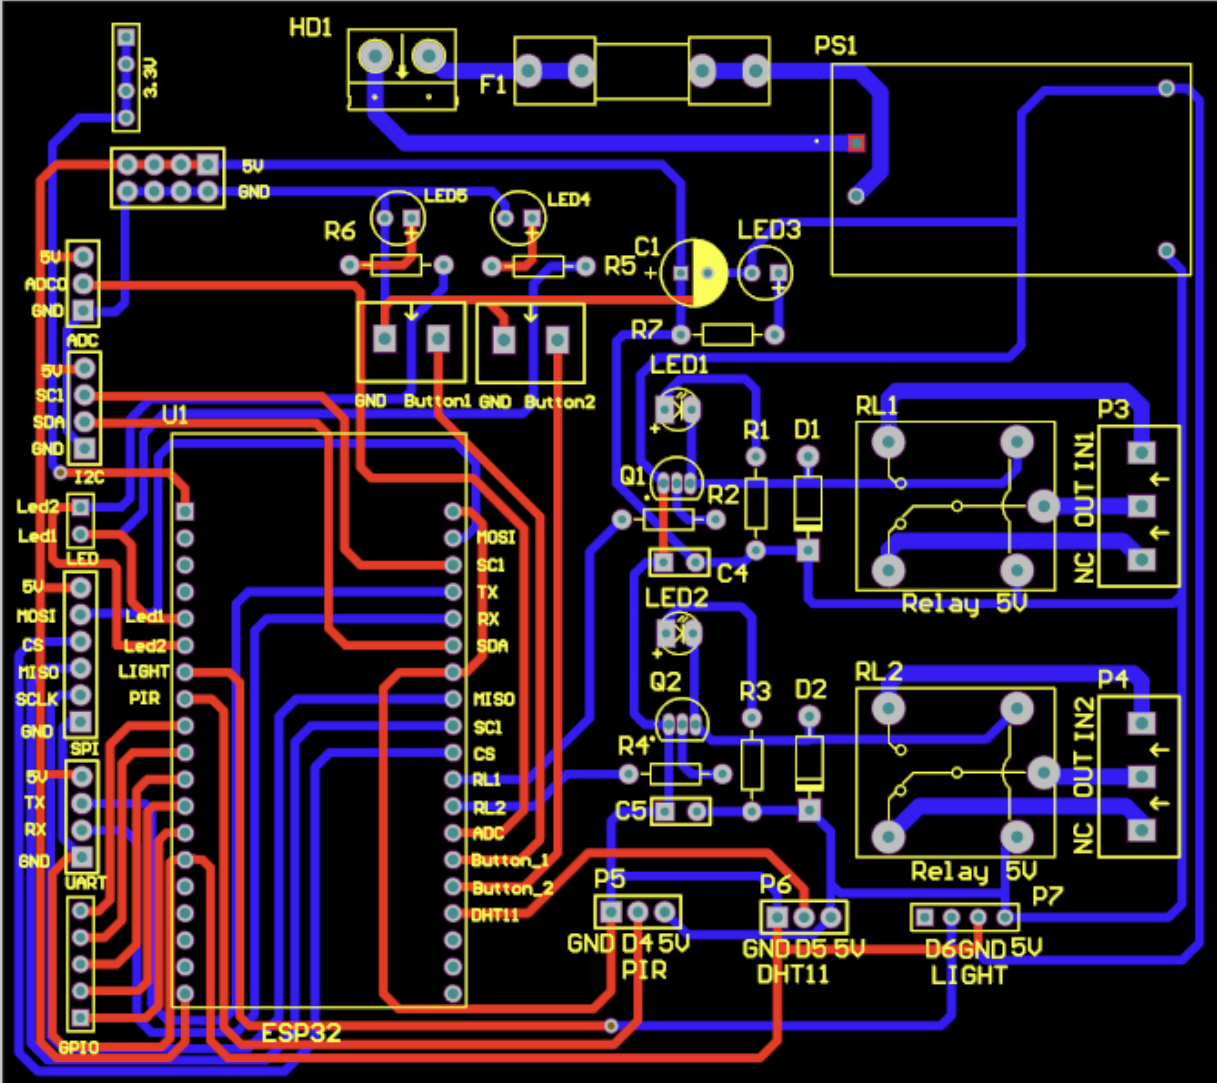
\includegraphics[width=\textwidth]{images/pcb_layout.png}
    \caption{Routed PCB layout (two-layer)}
    \label{fig:pcb_layout}
  \end{subfigure}
  \vspace{0.5em}
  \begin{subfigure}[b]{0.6\textwidth}
    \centering
    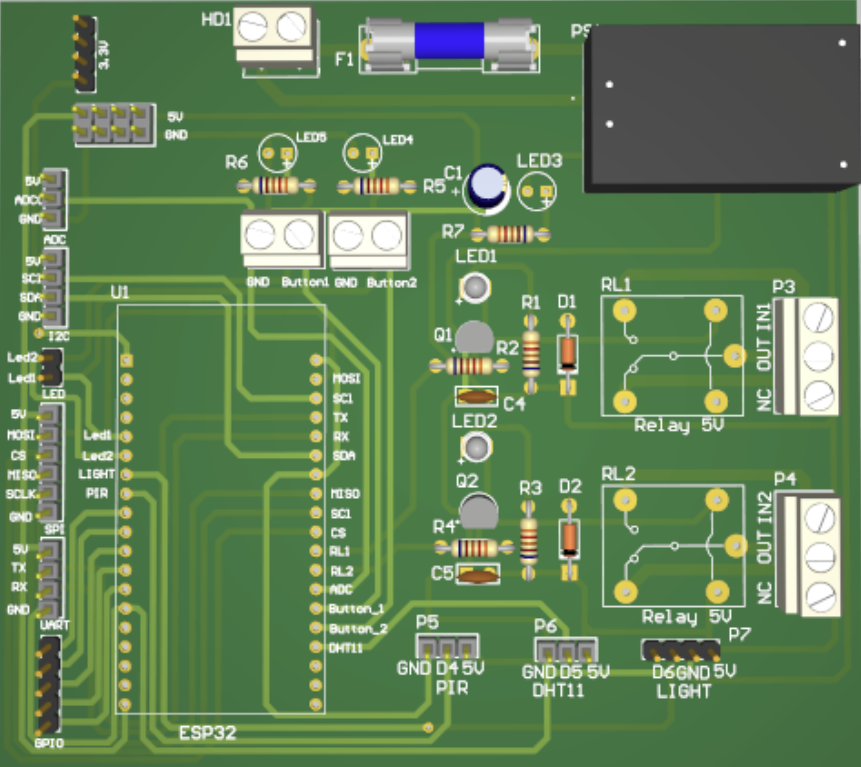
\includegraphics[width=\textwidth]{images/pcb_3d.png}
    \caption{3D render of the assembled PCB}
    \label{fig:pcb_3d}
  \end{subfigure}
  \caption[Two-layer PCB hardware platform]{Two-layer PCB used as the hardware platform (from prior coursework).}
  \label{fig:pcb_all}
\end{figure}

\FloatBarrier

% ─────────────────────────────────────────────────────────────
\section{Data Acquisition and Preprocessing}
\label{sec:data_method}

\subsection{Sensor Data Flow}

Environmental sensors (DHT11, LDR, PIR) publish readings every five seconds to the EMQX Cloud MQTT broker over TLS. Heart-rate data from the Coospo~H6 is streamed via the Python BLE bridge at approximately 1\,Hz. All messages are delivered to the Flask backend through wildcard subscriptions.
(\texttt{home/sensors/\#}~and~\texttt{home/status/\#}), parsed, and persisted
to MySQL through the SQLAlchemy ORM.

\subsection{Preprocessing Pipeline}

Before being fed into the machine learning pipeline, the data goes through the following steps:
    \begin{enumerate}
    \item \textbf{LDR normalisation}: the 12-bit ADC raw value (0--4095) is mapped to a 0--100 light intensity scale.
    \item \textbf{PIR edge filtering}: record only state-change events (DETECTED~$\leftrightarrow$~CLEAR) to prevent duplicate entries.
    \item \textbf{Heart-rate throttling}: a per-user 60-second write throttle, protected by a \texttt{threading.Lock}, ensures no concurrent database writes during continuous BPM streaming.
    \item \textbf{Temporal feature derivation}: from each UTC server
    timestamp the system derives \texttt{hour} (0--23), \texttt{is\_night}
    ($= 1$ if $20 \leq \text{hour}$ or $\text{hour} \leq 6$), and
    \texttt{is\_dark} ($= 1$ if light\_level $< 50$), providing circadian
    and environmental context to the anomaly pipeline.
    \item \textbf{Feature standardisation}: heart-rate values are normalised
    using a dedicated \texttt{StandardScaler}
    (\texttt{anomaly\_hr\_scaler.pkl}) before Isolation Forest inference.
\end{enumerate}

% ─────────────────────────────────────────────────────────────
\section{Technology Selection and Design Decisions}
\label{sec:tech_selection}

This section summarizes the major technology decisions that define the platform and the rationale for them, so that the designs for each component in the following sections can be read against a single set of decisions. The selection of each component is motivated by the elderly-care requirements (Section~\ref{sec:user_req}), i.e. low cost, low power, real-time responsiveness, data privacy and an accessible bilingual interface, and the gaps identified in the literature review. In Table~\ref{tab:tech_decisions}, the selected technologies, the main alternatives considered and the deciding rationale are summarized. The most consequential choices are elaborated in the remainder of this chapter.

\begin{table}[p]
\centering
\caption[Technology selections and design decisions]{Summary of technology selections and design decisions}
\label{tab:tech_decisions}
\footnotesize
\renewcommand{\arraystretch}{1.05}
\setlength{\tabcolsep}{4pt}
\begin{tabularx}{\textwidth}{@{} >{\raggedright\arraybackslash}p{2.5cm} >{\raggedright\arraybackslash}p{3.0cm} >{\raggedright\arraybackslash}p{2.6cm} >{\raggedright\arraybackslash}X @{}}
\toprule
\textbf{Concern} & \textbf{Selected} & \textbf{Alternatives} & \textbf{Deciding rationale} \\
\midrule
Microcontroller & ESP32-WROOM-32 & Arduino Uno, Raspberry Pi &
  \begin{tblitem}
    \item Dual-core with integrated Wi-Fi and BLE.
    \item Low unit cost and power draw.
    \item Sufficient GPIO headroom for sensor sampling and TLS MQTT.
  \end{tblitem} \\
\addlinespace[4pt]
Device messaging & MQTT over TLS & HTTP polling, CoAP &
  \begin{tblitem}
    \item Lightweight publish/subscribe, low overhead on constrained devices.
    \item Broker-mediated decoupling between sensor nodes and the backend.
  \end{tblitem} \\
\addlinespace[4pt]
Wearable HR link & Bluetooth Low Energy & Classic Bluetooth, ANT+ &
  \begin{tblitem}
    \item Low-power Heart Rate Service profile.
    \item Natively supported by ESP32 and host laptop; ANT+ requires a proprietary USB receiver.
  \end{tblitem} \\
\addlinespace[4pt]
Backend framework & Flask & FastAPI, Django &
  \begin{tblitem}
    \item Lightweight WSGI Python framework.
    \item FastAPI's async model conflicts with Flask-SocketIO threading and synchronous SQLAlchemy.
  \end{tblitem} \\
\addlinespace[4pt]
Backend structure & Modular layered & Monolithic MVC &
  \begin{tblitem}
    \item Separates domain, use-case, AI, gateway, infrastructure, and presentation concerns into distinct packages.
    \item Enables independent testing and replacement of individual components (Section~\ref{sec:arch_method}).
  \end{tblitem} \\
\addlinespace[4pt]
Web dashboard & Vite + Vanilla JS & React, Vue &
  \begin{tblitem}
    \item Direct control of the interactive floor-plan rendering without the overhead of a heavier SPA framework.
  \end{tblitem} \\
\addlinespace[4pt]
Mobile application & Flutter & React Native, native &
  \begin{tblitem}
    \item Single Dart codebase targeting both Android and iOS with a consistent user experience; the build was validated on Android in this work.
  \end{tblitem} \\
\addlinespace[4pt]
Anomaly detection & Isolation Forest (heart-rate only) & One-Class SVM, autoencoders, fixed threshold &
  \begin{tblitem}
    \item Unsupervised one-class model; no labelled anomalies required.
    \item Full algorithm comparison in Section~\ref{subsec:ml_selection}.
    \item Sub-millisecond inference confirmed in Section~\ref{subsec:latency_protocol}.
  \end{tblitem} \\
\addlinespace[4pt]
Conversational AI & Tri-modal: Rule, Ollama qwen2.5:3b, Gemini & Cloud-only LLM &
  \begin{tblitem}
    \item Local rule and on-device LLM paths preserve privacy and enable offline fallback.
    \item Cloud path (Gemini Flash) adds open-ended capability (Section~\ref{sec:alfred_method}).
  \end{tblitem} \\
\bottomrule
\end{tabularx}
\end{table}
% ─────────────────────────────────────────────────────────────
\section{System Architecture Design}
\label{sec:arch_method}

\subsection{Four-Tier Architecture and Physical Deployment}
\label{subsec:deployment}

The platform uses a four-tier IoT architecture, with communication
following a unidirectional data flow from the hardware layer upward to the
presentation layer:

\begin{itemize}
    \item \textbf{Hardware layer.} The ESP32 node collects environmental and physiological signals and controls relay actuators. A Python BLE bridge handles heart-rate data from the Coospo H6 wearable.

    \item \textbf{Communication layer.} An EMQX Cloud MQTT broker acts as the main message hub. All sensor telemetry and device-control commands are transmitted over TLS-secured connections.

    \item \textbf{Backend layer.} A Python Flask service receives incoming sensor data, stores it in MySQL, runs the anomaly detection pipeline, exposes REST endpoints and Socket.IO events, while also hosting the Alfred AI assistant.

    \item \textbf{Presentation layer.} A Vite-based web dashboard and a Flutter mobile app form the caregiver-facing front end for monitoring, device control, health data review, and natural-language interaction.\end{itemize}

Figure~\ref{fig:deployment} shows how these four logical tiers map onto the
physical nodes of the prototype deployment. All \emph{software} services
(Flask, MySQL, Ollama, BLE bridge) run on a single developer laptop
(Windows, 16\,GB RAM). The ESP32 node and Coospo~H6 are physical hardware
devices on the local network; EMQX Cloud and Google Gemini are the primary
external cloud dependencies.

\begin{landscape}
\begin{figure}[p]
\centering
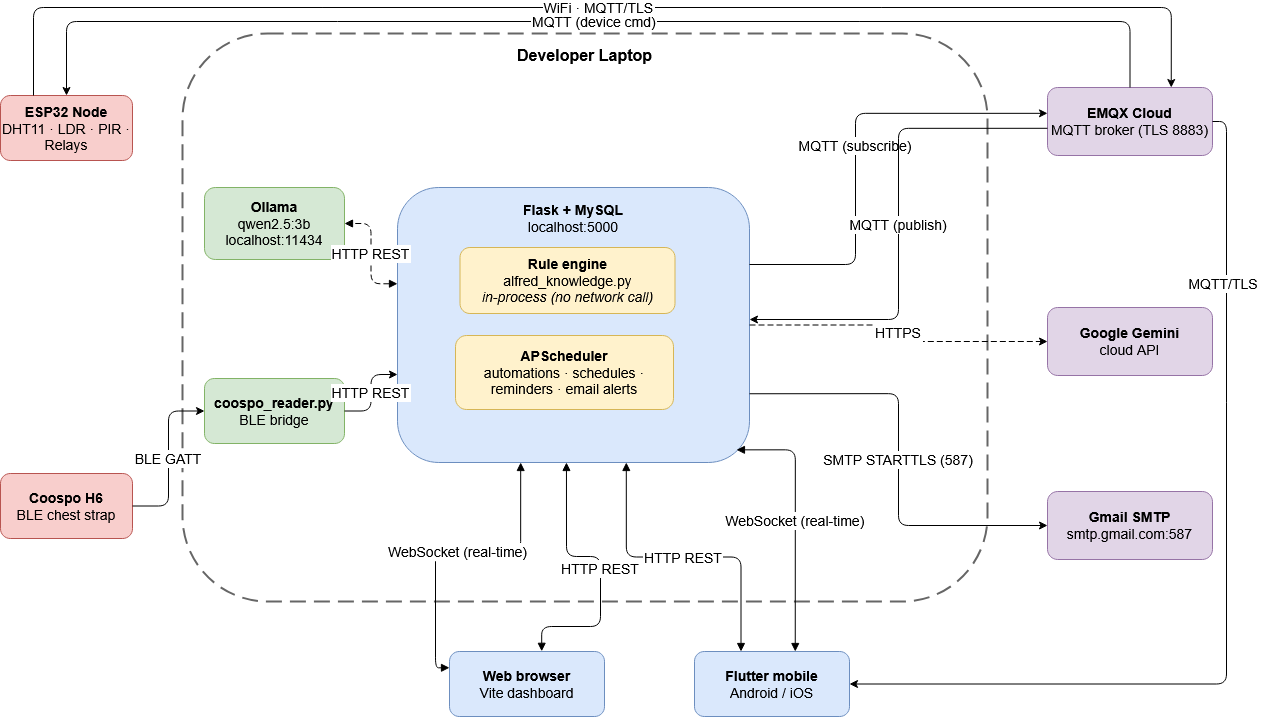
\includegraphics[width=\linewidth,height=0.80\textwidth,keepaspectratio]{images/deployment.png}
\caption[Physical deployment and four-level IoT architecture]
{Four-level IoT architecture and physical deployment. The Flask services are running on the developer laptop, and the ESP32 node and Coospo~H6 are physical devices on the local network. The Rule Engine is in-process and runs inside Flask. Ollama and Gemini are conditionally used based on Alfred mode. Optional communication paths are indicated by dashed arrows. The primary external cloud services are EMQX Cloud and Google Gemini.}
\label{fig:deployment}
\end{figure}
\end{landscape}

\FloatBarrier

\subsection{Backend Modular Structure}

The Flask backend is organised into six functional modules, each responsible for a distinct concern. Dependency injection is managed in \texttt{app/wiring.py} using a \texttt{dependency\_injector} container that wires components together at startup.

\begin{itemize}[itemsep=4pt, parsep=0pt, topsep=4pt]

    \item \textbf{Domain} (\texttt{app/domain/}): Core data models (\texttt{Device}, \texttt{Status}, \texttt{Log}) and abstract port interfaces (\texttt{publisher}, \texttt{email\_notifier}, \texttt{realtime}). No framework imports.

    \item \textbf{Use Cases} (\texttt{app/usecases/}): Orchestration of business logic --- \texttt{DeviceUseCase}, \texttt{AlertUseCase}, \texttt{AIUseCase}, and others --- coordinating between repositories, gateways, and AI services.

    \item \textbf{AI / ML} (\texttt{app/ai/}): Isolation Forest anomaly detection, mood prediction, HRV analysis, and feature engineering. The heart-rate coordination service (\texttt{heart\_rate\_ai.py}) is the central pipeline that integrates inference results with persistence, real-time notification, and alert dispatch.

    \item \textbf{Gateways} (\texttt{app/gateways/}): Protocol adapters that connect external communication channels to the application --- MQTT publisher/listener, Socket.IO emitter, and email notifier.

    \item \textbf{Infrastructure} (\texttt{app/infrastructure/}): SQLAlchemy ORM models and MySQL repository implementations providing persistence for all entities.

    \item \textbf{Presentation} (\texttt{app/presentation/api/}): Flask blueprints exposing REST endpoints and Socket.IO events to the web dashboard and mobile app.

\end{itemize}

Figure~\ref{fig:clean_arch} illustrates the module hierarchy from the most protocol-facing layer (Presentation) down to the framework-independent Domain.

\begin{figure}[H]
\centering
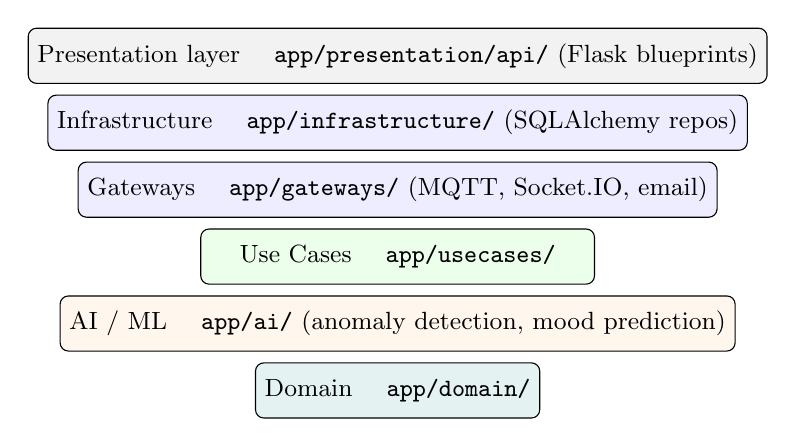
\begin{tikzpicture}[
  layer/.style={draw, minimum width=#1, minimum height=0.7cm,
                align=center, font=\small, rounded corners=3pt},
  lbl/.style={font=\scriptsize, align=left},
]
\def\w{9.2cm}
\node[layer=\w, fill=gray!10]     (pres) at (0, 0)    {Presentation layer \quad \texttt{app/presentation/api/} (Flask blueprints)};
\node[layer=7.8cm, fill=blue!7]   (infra)at (0,-0.85) {Infrastructure \quad \texttt{app/infrastructure/} (SQLAlchemy repos)};
\node[layer=6.4cm, fill=blue!7]   (gw)   at (0,-1.70) {Gateways \quad \texttt{app/gateways/} (MQTT, Socket.IO, email)};
\node[layer=5.0cm, fill=green!8]  (uc)   at (0,-2.55) {Use Cases \quad \texttt{app/usecases/}};
\node[layer=3.6cm, fill=orange!7] (ai)   at (0,-3.40) {AI / ML \quad \texttt{app/ai/} (anomaly detection, mood prediction)};
\node[layer=2.2cm, fill=teal!10]  (dom)  at (0,-4.25) {Domain \quad \texttt{app/domain/}};
\end{tikzpicture}
\caption[Flask backend module hierarchy]{Flask backend module hierarchy. Modules are grouped by responsibility from the protocol-facing Presentation layer down to the framework-independent Domain. The AI/ML module handles the full heart-rate processing pipeline including inference, persistence, and real-time alerting.}
\label{fig:clean_arch}
\end{figure}

\FloatBarrier

\subsection{Database Schema Design}

The system uses MySQL~8.0, managed by SQLAlchemy, and is divided into three entity modules: Auth, Health, and Device. Table~\ref{tab:db} summarises the
core tables; the complete entity-relationship diagram is presented in
Figure~\ref{fig:erd_full}.

\begin{table}[H]
\centering
\caption{Core database tables grouped by module}
\label{tab:db}
\small
\begin{tabularx}{\textwidth}{@{} l >{\RaggedRight\arraybackslash}X @{}}
\toprule
\textbf{Module / Table} & \textbf{Purpose} \\
\midrule
\multicolumn{2}{@{}l}{\textit{Auth module}} \\
\quad\texttt{users}                    & Accounts, hashed passwords, role (\texttt{admin}/\texttt{user}/\texttt{guest}) \\
\quad\texttt{password\_reset\_tokens}  & Time-limited reset codes (hashed, 30-min expiry) \\
\quad\texttt{alert\_mute\_preferences} & Per-user alert visibility mute scope and keyword \\
\quad\texttt{alert\_saved\_view\_configs} & Persisted alert filter presets (level, device, date range) per user \\
\midrule
\multicolumn{2}{@{}l}{\textit{Health module}} \\
\quad\texttt{patient\_profiles}   & Name, age, gender, baseline HR, diagnosis notes, medications \\
\quad\texttt{patient\_hr\_records}& BPM, severity, risk level, mood label \\
\quad\texttt{medicine\_reminders} & Medicine name, dosage, time, recurrence pattern, active flag \\
\midrule
\multicolumn{2}{@{}l}{\textit{Device module}} \\
\quad\texttt{rooms}         & Room name, polygon JSON, floor-plan URL \\
\quad\texttt{device}        & Device code, category, room assignment, map coordinates \\
\quad\texttt{device\_status}& Latest ON/OFF state and value per device \\
\quad\texttt{sensor\_data}  & Time-series sensor readings \\
\quad\texttt{control\_log}  & Audit trail of all device commands \\
\quad\texttt{alerts}        & Anomaly events with severity and read state \\
\quad\texttt{notifications} & Per-user in-app notification records (title, body, read state) linked to an alert \\
\quad\texttt{alert\_rules}  & Threshold rules per device/sensor type \\
\quad\texttt{schedules}     & Cron-based scheduled device actions \\
\quad\texttt{automations}   & Trigger-action pairs for conditional automation \\
\bottomrule
\end{tabularx}
\end{table}

The alert-visibility mute feature is persisted in the dedicated \texttt{alert\_mute\_preferences} table, and the backend restores the saved scope and keyword when the user comes back on another device. A dedicated repair script \texttt{backend/migrate\_alert\_mute\_preferences.py} creates the table if it does not exist, and safely adds the required columns and indexes if the schema is incomplete.

\begin{landscape}
\begin{figure}[p]
\centering
% In an lscape landscape page the visual height corresponds to \textwidth.
% Cap the image well below \textwidth so the multi-line caption also fits
% on the same rotated page.
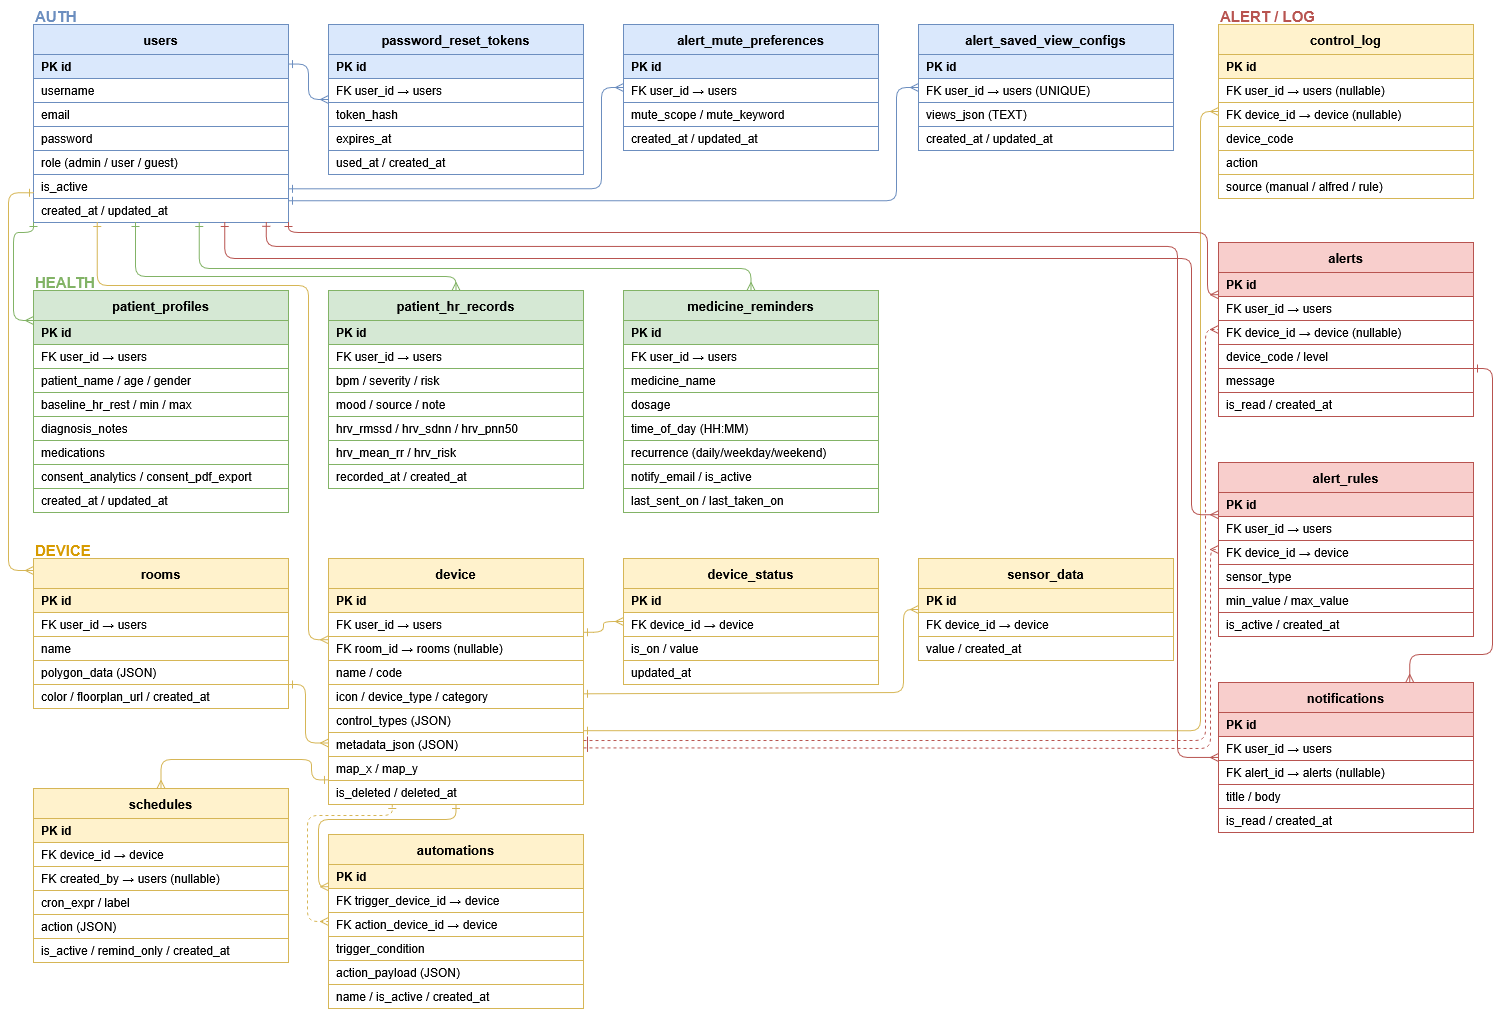
\includegraphics[width=\linewidth,height=0.80\textwidth,keepaspectratio]{images/erd_full.png}
\caption[Database entity-relationship diagram]{Complete database schema (17
  tables). \emph{Auth}: \texttt{users}, \texttt{password\_reset\_tokens},
  \texttt{alert\_mute\_preferences}, \texttt{alert\_saved\_view\_configs}.
  \emph{Health}: \texttt{patient\_profiles}, \texttt{patient\_hr\_records},
  \texttt{medicine\_reminders}. \emph{Device Core}: \texttt{rooms},
  \texttt{device}, \texttt{device\_status}, \texttt{sensor\_data},
  \texttt{control\_log}. \emph{Device Events}: \texttt{alerts},
  \texttt{alert\_rules}, \texttt{notifications}, \texttt{schedules},
  \texttt{automations}.}
\label{fig:erd_full}
\end{figure}
\end{landscape}


\subsection{Authentication and Role-Based Access Control}
\label{subsec:rbac}

The platform defines two active roles: \texttt{admin} and \texttt{user} (the default). A \texttt{guest} role exists in the schema for future caregiver-observer workflows but is not yet activated. Admins can configure accounts, assign automation rules --- for example, triggering a fan when temperature exceeds 40\,°C --- and act on behalf of any patient. Regular users see only their own sensor data, alerts, schedules, and AI outputs.

Tokens are signed with \texttt{itsdangerous.URLSafeTimedSerializer} on a 7-day TTL and verified without a database round-trip: the \texttt{@auth\_required} decorator checks the signature and loads \texttt{g.current\_user} straight from the token payload. How the token travels depends on the client. The web dashboard keeps it in an \texttt{HttpOnly} cookie (\texttt{SameSite=Strict}) so JavaScript cannot read it; the Flutter app sends it as a \texttt{Bearer} header on every request, since Dart's HTTP layer has no cookie jar. A separate \texttt{@admin\_required} decorator guards any endpoint that regular users should not reach and returns \texttt{403} on a role mismatch.

Data isolation is enforced at three levels. Every ORM query filters by \texttt{user\_id}. Route handlers re-verify ownership before returning a resource and respond with \texttt{404} rather than \texttt{403} so that the existence of another user's record is not leaked. Real-time events are confined to per-user Socket.IO rooms (\texttt{user\_\{id\}}), so a patient's sensor alerts and AI replies never cross into another active session.

\clearpage

% ─────────────────────────────────────────────────────────────
\section{User Interface Design}
\label{sec:ui_method}

\subsection{Web Dashboard Layout}

The web dashboard is a single page application (Vite/ES6 modules). It is divided into 7 pages, with a persistent sidebar (the Admin page is hidden for non-admin users):
\begin{itemize}[itemsep=4pt, parsep=0pt, topsep=4pt]
    \item \textbf{Dashboard}: A unified home view that brings together key patient and system information, including real-time vital signs, weather updates, schedule overview, active alerts, and AI-based health insights generated by Alfred, along with quick access to device controls.

    \item \textbf{Health Monitor}: A real-time monitoring interface for visualizing heart rate trends, anomaly risk flags, and AI-generated mood labels retrieved from the backend via Socket.IO and REST endpoints.

    \item \textbf{Floor-Plan Editor}: A visual editor that allows caregivers to define room layouts from uploaded floor-plan images by drawing room boundaries, assigning devices, and managing multiple floors.

    \item \textbf{Alert Management}: A centralized system for tracking and managing alerts with severity-based filtering and user-defined mute rules. Critical events, including SOS alerts triggered by detected distress signals from the AI system, are recorded and automatically sent to caregivers.

    \item \textbf{Care and Schedule}: A calendar-based module for managing daily activities, medications, and device automation. It supports multiple views and allows caregivers to define time-based actions using cron-like scheduling.

    \item \textbf{Health Report}: A reporting module that generates daily and weekly summaries of patient status, including vital signs, alert history, medication adherence, and AI analysis, with support for export via print or email.

    \item \textbf{Admin} (role-gated): A restricted area for managing caregiver accounts, assigning patients, and handling role-based access control.
\end{itemize}

Figure~\ref{fig:method_dashboard_layout} depicts the main Dashboard , and screenshots of the remaining views are presented in Chapter~4.

\begin{figure}[htbp]
\centering
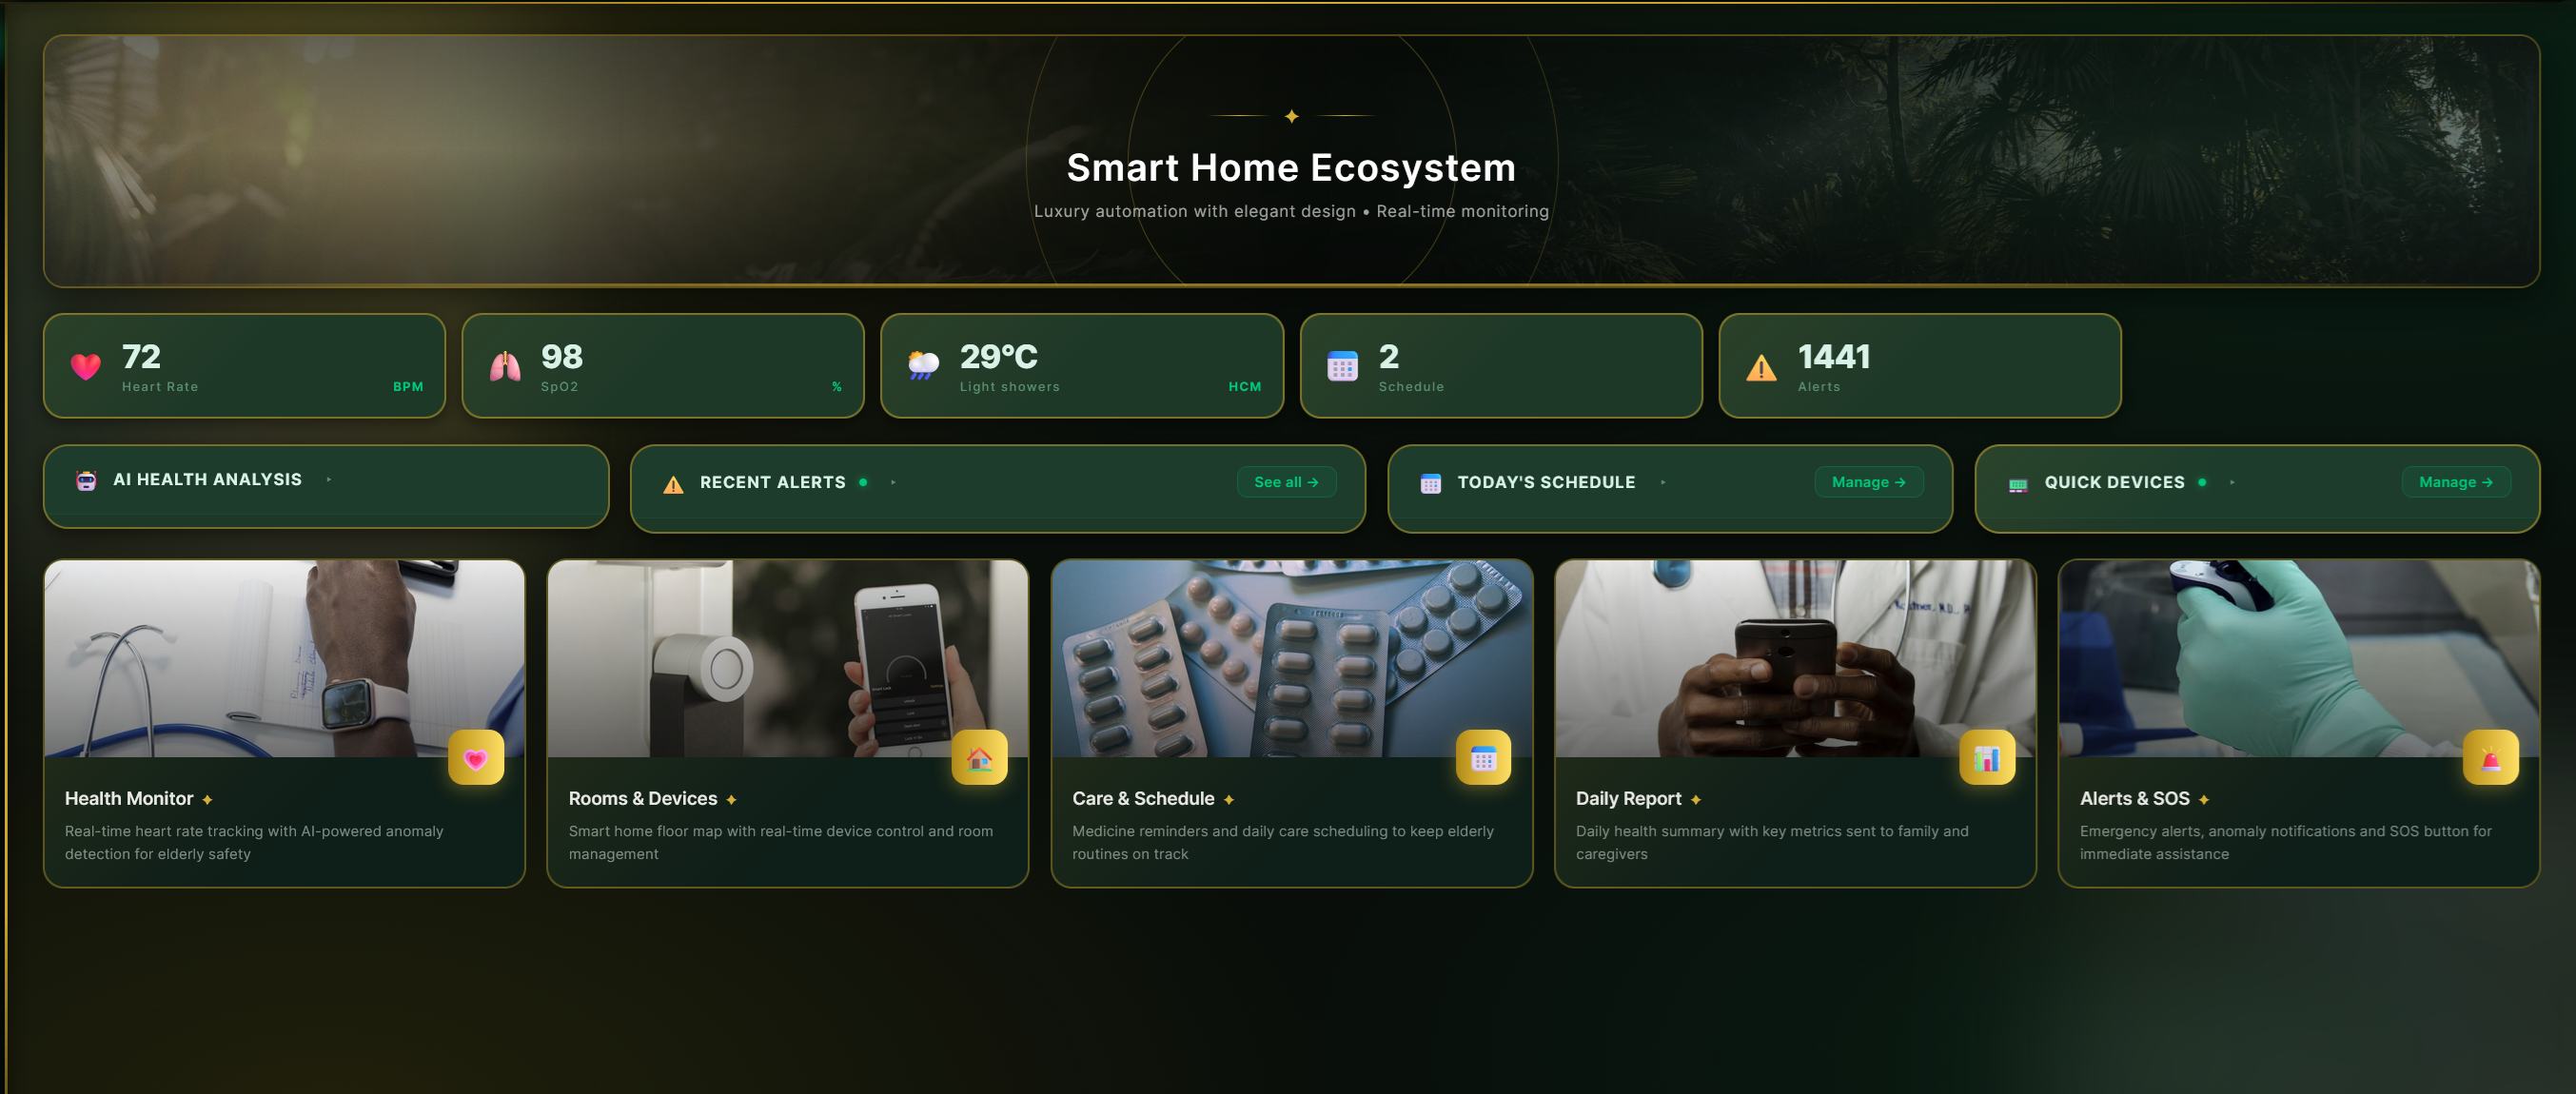
\includegraphics[width=0.92\textwidth]{images/web_dashboard.png}
\caption[Web dashboard layout]{Web dashboard layout showing the live sensor tiles, real-time
  heart-rate chart, device toggle grid, and Alfred chat terminal.}
\label{fig:method_dashboard_layout}
\end{figure}

\subsection{Room Configuration and Device Management Workflow}
\label{subsec:room_device_workflow}

Room and device management follows a three-stage workflow: (1)~an admin registers a device by specifying its \texttt{device\_code} (the MQTT topic identifier), category (\texttt{relay}/\texttt{sensor}/\texttt{camera}), and optional room assignment; (2)~the caregiver traces room polygons on an HTML5 canvas overlay of the uploaded floor-plan image, with vertex coordinates stored as image-fraction values to ensure resolution independence; (3)~devices are placed on the map using a two-click interaction, after which the backend automatically assigns each marker to the corresponding room polygon using a point-in-polygon test. All changes are pushed via Socket.IO to connected clients, and the mobile app displays the same floor-plan in read-only mode. The dialog for defining the zone and the resulting polygon overlay are shown in Figure~\ref{fig:floorplan_editor_full} (Chapter~\ref{chap:experiments}).

\subsection{Mobile Application Screen Structure}

The Flutter mobile application consists of eight screens: six of which can be reached through a bottom navigation bar (Control, Routines, Alfred, Health, Alerts, Map) and Settings and Login. Figure~\ref{fig:mobile_nav} illustrates the
navigation structure. Implementation details and screenshots are presented in
Section~\ref{sec:mobile_impl}.

\begin{figure}[htbp]
\centering
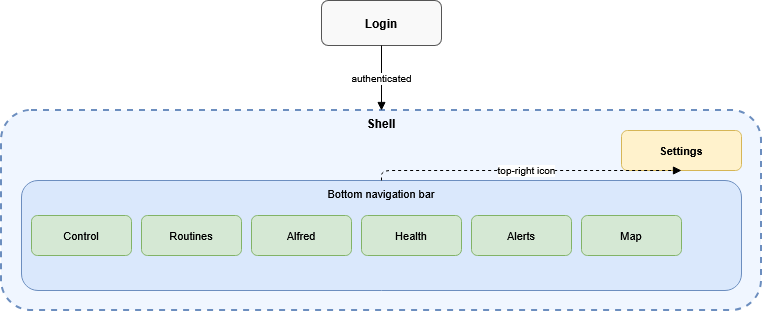
\includegraphics[width=0.85\textwidth]{images/mobile_nav.png}
\caption[Navigation structure of the Flutter mobile application]{The Flutter mobile application navigation starts from the Login screen, leading to a main bottom navigation bar with six tabs, and further to the Settings screen. Users can access Settings from any tab via the top-right icon.}
\label{fig:mobile_nav}
\end{figure}

\FloatBarrier

\subsection{Care and Schedule Page Design}
\label{subsec:reminder_calendar}

The web dashboard features a \textbf{Care \& Schedule} page with a Google Calendar-style~\cite{GoogleCalendar2024} interface supporting four colour-coded event categories: Medicine (blue), Activity (purple), Appointment (green), and Note (pink), with Month, Week, and Day view modes. The Day view features a medicine adherence progress bar and per-event Done/Edit controls, while overdue medicines are highlighted in amber. Medicine reminders (those with a fixed time and recurrence) are persisted to the backend through \texttt{/api/reminders}, enabling cross-device synchronisation. Other calendar entries (Activity, Appointment, Note) are stored in browser \texttt{localStorage} keyed by user ID. Client-side conflict detection identifies any two events that share the same HH:MM slot within a day column. It highlights the affected cards and column header in amber without requiring an additional backend query. The mobile \textbf{Routines} screen mirrors this with a horizontally scrollable 7-column weekly grid. The Month view is shown in Figure~\ref{fig:method_care_page}.


\begin{figure}[htbp]
\centering
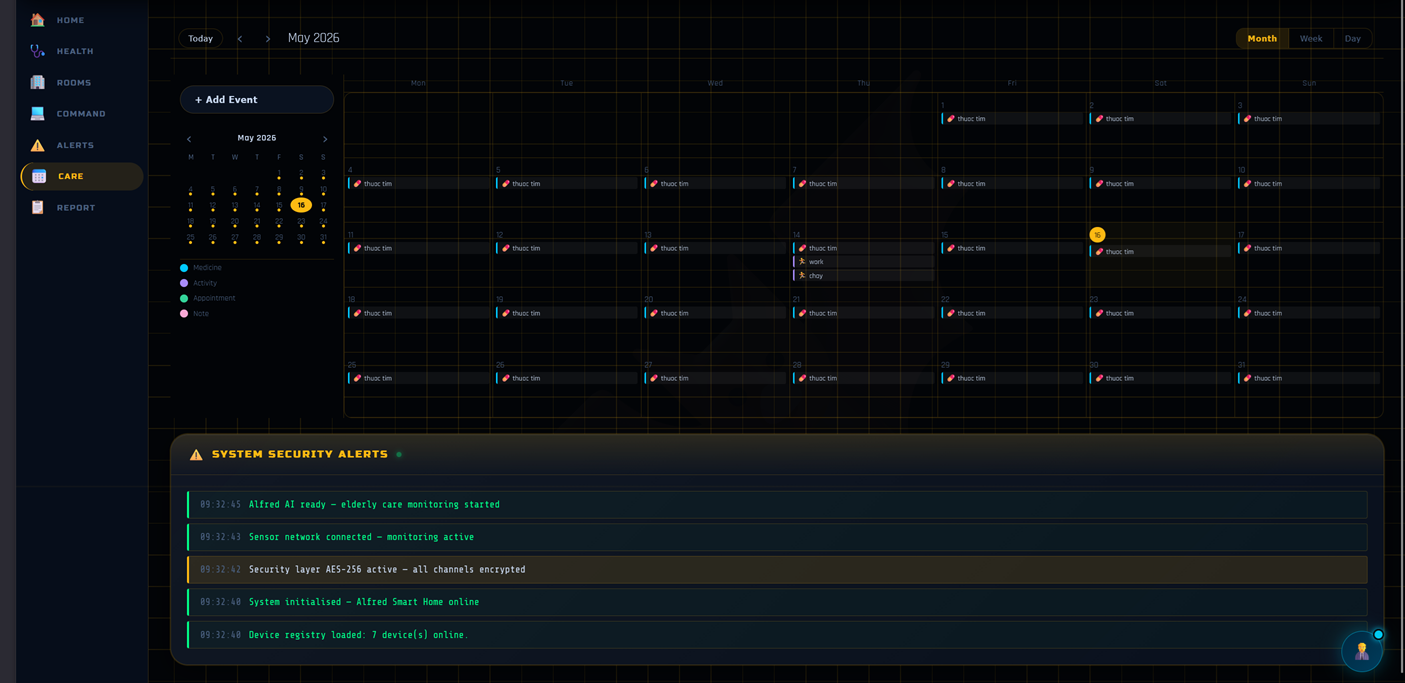
\includegraphics[width=0.90\textwidth]{images/web_care.png}
\caption[Care \& Schedule page: Month view with colour-coded event categories]{Care \& Schedule page in Month view (May 2026): monthly calendar grid displaying recurring medicine events (\textit{thuốc tim}) across all days, with activity events colour-coded by category (Medicine blue, Activity purple, Appointment green, Note pink). Left sidebar provides an Add Event button, mini calendar navigation, and legend.}
\label{fig:method_care_page}
\end{figure}

\subsection{Health Report Design}
\label{subsec:report_design}

The Report page generates two on-demand, print-optimised HTML reports.

The \textbf{Daily Report} gives a snapshot of caregiver handover, summarizing key daily metrics like medication adherence, schedule completion, and alert count, along with detailed tables of medications, events, and alerts retrieved from the backend APIs.

The \textbf{Weekly Report} gives a more general overview of the patient’s physiological state over a seven-day period, including vital-sign statistics, AI-based cardiac assessment from Alfred, alert severity distribution, and clinical notes.

Both reports open in a browser popup and are automatically sent to the print dialog via \texttt{window.print()} (Figure~\ref{fig:method_health_report}).

\begin{figure}[htbp]
\centering
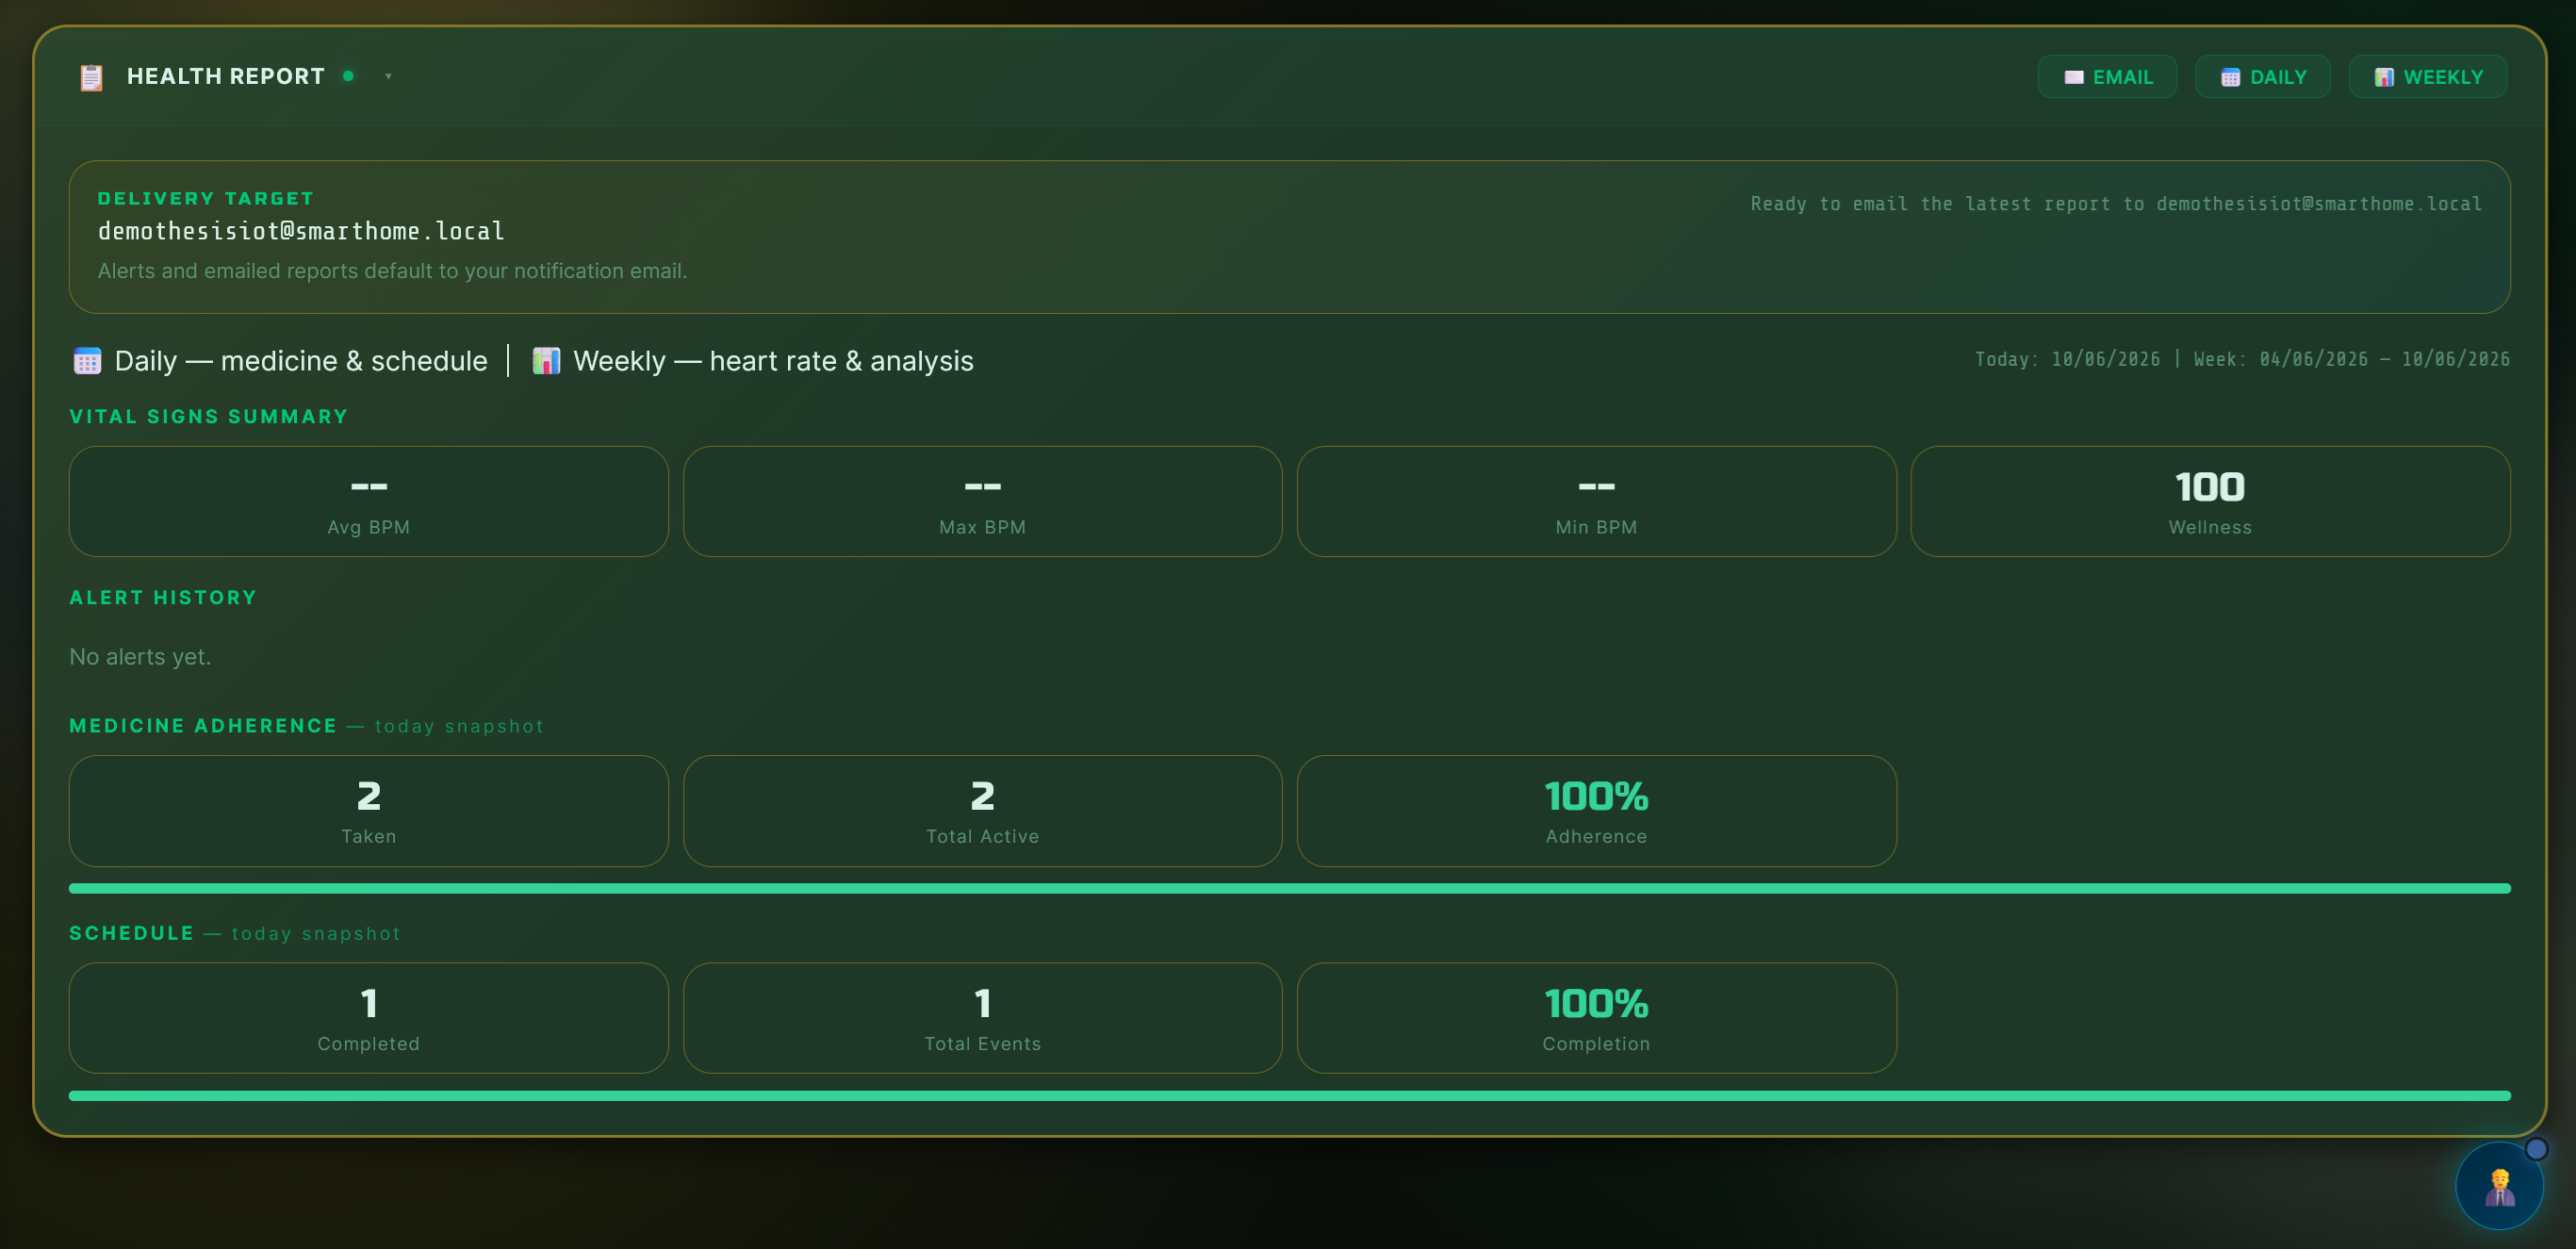
\includegraphics[width=0.82\textwidth]{images/fig_health_report_export_ui.png}
\caption[Health Report export interface]{Health Report export panel: delivery target, reporting period (weekly), vital signs summary (Avg BPM and Max BPM), alert history status, and EMAIL/PRINT export controls.}
\label{fig:method_health_report}
\end{figure}

% ─────────────────────────────────────────────────────────────
\section{Intelligent Health Analytics and AI Assistant Design}
\label{sec:ml_method}

\subsection{Heart-Rate Anomaly Detection}
\label{sec:anomaly_design}

\paragraph{Algorithm Selection Rationale}

Monitoring of the elderly requires detection of health anomalies using a method that does not rely on labelled anomaly data as real cardiac events are rare and difficult to collect ethically. The model should also support near real-time inference (under 100\,ms) and integrate naturally with a Python scikit-learn pipeline~\cite{Pedregosa2011}.

\textbf{Isolation Forest} \cite{Liu2008} was selected as it satisfies these constraints. It was preferred over the other candidate methods reviewed in Section~\ref{subsec:ml_selection} (One-Class SVM, and LSTM and dense autoencoders), which have more complex hyperparameter spaces, are slower to retrain on streaming data, and offer no clear accuracy advantage for the single-feature cardiac signal used here. The deployed Isolation Forest is benchmarked empirically against a simple fixed-threshold baseline in Section~\ref{sec:ml_validation} (Table~\ref{tab:feature_ablation}).

\paragraph{Feature Selection}

Seven candidate features are defined in the shared configuration:

\begin{enumerate}
    \item \textbf{heart\_rate} --- beats per minute from the Coospo~H6.
    \item \textbf{room\_temp} --- ambient temperature ($^\circ$C) from DHT11.
    \item \textbf{humidity} --- relative humidity (\%) from DHT11.
    \item \textbf{light\_level} --- normalised ambient light (0--100) from LDR.
    \item \textbf{hour} --- integer hour of day (0--23) for circadian context.
    \item \textbf{is\_night} --- binary: 1 if $20 \leq \text{hour}$ or $\text{hour} \leq 6$.
    \item \textbf{is\_dark} --- binary: 1 if light\_level $< 50$.
\end{enumerate}

In preliminary experiments, model performance was worse when all seven features were included. This is because each tree randomly samples from all features, making the probability of selecting \texttt{heart\_rate} only 1-in-7, which dilutes the cardiac anomaly signal. The deployed model therefore uses \textbf{heart\_rate} as its sole input. The remaining six features remain in the shared configuration and can be activated if multi-modal monitoring is added later.

The contamination parameter is selected by a grid search over nine values $\{0.010,\,0.015,\,0.020,\,0.025,\,0.030,\,0.035,\,0.040,\,0.050,\,0.060\}$, evaluating precision, recall, and anomaly F1 on a held-out synthetic set of 2\,000 samples: 1\,900 normal and 100 anomaly (50 tachycardia HR~140--210, 30 bradycardia HR~15--37, 11 moderate tachycardia HR~100--135, and 9 in-range samples where HR is normal but context is anomalous --- these last 9 are structurally undetectable by an HR-only model and set a natural recall ceiling below~1.0). Table~\ref{tab:contamination_grid} reports the full results.

\begin{table}[H]
\centering
\caption[Production contamination grid search results]{Production contamination grid search: Isolation Forest trained on UCI-healthy~+~1\,700 synthetic normals (2\,099 samples), evaluated on the 2\,000-sample synthetic labelled set. Values $\geq 0.050$ show a sharp precision drop; \texttt{contamination}~=~0.020 is selected as a conservative choice within the high-precision range.}
\label{tab:contamination_grid}
\small
\begin{tabular}{@{} c c c c l @{}}
\toprule
\textbf{Contamination} & \textbf{Precision} & \textbf{Recall} & \textbf{F1} & \textbf{Note} \\
\midrule
0.010 & 1.00 & 0.90 & 0.95 & \\
0.015 & 1.00 & 0.90 & 0.95 & \\
\textbf{0.020} & \textbf{1.00} & \textbf{0.91} & \textbf{0.95} & \textbf{Selected} \\
0.025 & 1.00 & 0.91 & 0.95 & \\
0.030 & 1.00 & 0.93 & 0.96 & \\
0.035 & 1.00 & 0.93 & 0.96 & \\
0.040 & 1.00 & 0.93 & 0.96 & \\
0.050 & 0.74 & 0.93 & 0.82 & Precision drop \\
0.060 & 0.74 & 0.94 & 0.83 & Precision drop \\
\bottomrule
\end{tabular}
\end{table}

Values 0.010--0.040 all achieve precision~1.00, meaning no false alerts on normal readings within this synthetic test set. Among these, \texttt{contamination}~=~0.020 is retained for production: it sits in the middle of the high-precision band and produces a lower alert rate than higher values, which matters more in continuous home monitoring than squeezing out an extra percentage point of recall. Values $\geq 0.050$ flag roughly one in four normal readings as anomalous --- an alert rate that would quickly cause caregiver fatigue and was ruled out on that basis.

Note that Table~\ref{tab:contamination_grid} reports F1~=~0.95 for \texttt{contamination}~=~0.020, while the UCI held-out evaluation in Table~\ref{tab:feature_ablation} (Chapter~5) reports F1~=~0.51 for the same setting. The gap comes entirely from the test set: the synthetic set here is balanced (95\% normal, 5\% anomaly) and its anomaly BPM values were generated to be clearly outside the normal band, so the model separates them easily. The UCI cohort is 84\% diseased patients whose BPMs, after the thalach approximation, overlap more with the healthy range --- a harder and more clinically realistic problem.

\paragraph{Risk Classification Design}
\label{subsec:risk_design}

Each incoming BPM reading passes through a two-layer decision pipeline before a risk level is assigned (Table~\ref{tab:risk}):

\begin{enumerate}
    \item \textbf{Layer 1 — Hard threshold (always evaluated first).}
    If BPM~$<$~50, the reading is classified as Caution (bradycardia).
    If $100 \leq \text{BPM} < 130$, it is Warning (tachycardia onset);
    if BPM~$\geq$~130, it is Critical (severe tachycardia).
    These rules fire unconditionally --- no ML score is consulted.

    \item \textbf{Layer 2 — Isolation Forest (consulted only for BPM 50--99).}
    Readings that clear Layer~1 are passed to the IF anomaly scorer.
    Within the 50--99 range, only two \emph{borderline sub-zones} activate the
    IF score: 50--59\,bpm and 96--99\,bpm.
    If the IF flags a reading in either sub-zone as an outlier, it is
    elevated to Caution.
    Readings in the clearly normal zone (60--95\,bpm) are labelled Normal
    regardless of the IF score, to suppress false positives in that range.
\end{enumerate}

This two-layer design ensures that clinically extreme values (BPM~$<$~50 or $\geq$~100) are always captured even before the IF model has been trained on sufficient patient-specific data, while the IF adds a statistical second opinion for borderline readings that fall between the hard-threshold boundaries.

\begin{table}[H]
\centering
\caption[Heart-rate risk level thresholds]{Heart-rate risk level thresholds, clinical basis, and system actions}
\label{tab:risk}
\small
\begin{tabularx}{\textwidth}{@{} l >{\RaggedRight\arraybackslash}p{2.2cm}
                                   >{\hsize=1.1\hsize\RaggedRight\arraybackslash}X
                                   >{\hsize=0.9\hsize\RaggedRight\arraybackslash}X @{}}
\toprule
\textbf{Level} & \makecell[l]{\textbf{BPM}\\\textbf{range}} & \textbf{Clinical basis} & \textbf{System action} \\
\midrule
Normal   & 50--99 &
  \begin{tblitem}
    \item AHA resting HR guideline: 60--100\,bpm~\cite{AHA2024}.
    \item Lower bound extended to 50\,bpm for physically active elderly.
  \end{tblitem} &
  \begin{tblitem}
    \item No alert.
    \item Reading persisted.
  \end{tblitem} \\
\addlinespace[4pt]
Caution  & $<50$; or IF outlier in borderline zone (50--59 or 96--99\,bpm) & Bradycardia (AHA)~\cite{AHA2024}; or borderline reading flagged as Isolation Forest outlier. IF outliers in the clearly normal zone (60--95\,bpm) are suppressed to avoid false positives. &
  \begin{tblitem}
    \item Alert logged.
    \item Socket.IO \mbox{\texttt{hr\_alert}} emitted.
  \end{tblitem} \\
\addlinespace[4pt]
Warning  & 100--129 & Tachycardia onset (AHA)~\cite{AHA2024}. &
  \begin{tblitem}
    \item Alert + Socket.IO push.
    \item Toast notification.
  \end{tblitem} \\
\addlinespace[4pt]
Critical & $\geq 130$ &
  \begin{tblitem}
    \item Severe tachycardia.
  \end{tblitem} &
  \begin{tblitem}
    \item Immediate alert, audio chime.
    \item In-app critical banner.
  \end{tblitem} \\
\bottomrule
\end{tabularx}
\end{table}

The threshold of 130 bpm for the Critical level is conservatively set below the commonly cited severe tachycardia threshold of 150 bpm to enable earlier caregiver intervention for elderly users who may tolerate rapid heart rates less well than younger adults.

\paragraph{Isolation Forest Anomaly Score}
\label{subsec:if_score}

The Isolation Forest algorithm computes an anomaly score $s(x,n)$ for each input $x$ based on the average path length $E[h(x)]$ across $T$ isolation trees, where $n$ is the subsampling size:

\begin{equation}
s(x,\,n) \;=\; 2^{-\,\dfrac{E[h(x)]}{c(n)}}
\label{eq:if_score}
\end{equation}

\noindent where $c(n)$ (Equation~\eqref{eq:cn}) represents the expected path length of an unsuccessful search in a binary search tree of $n$ nodes:

\begin{equation}
c(n) \;=\; 2\,H(n-1) - \dfrac{2(n-1)}{n},
\qquad H(i) = \ln i + 0.5772
\label{eq:cn}
\end{equation}
A score $s \to 1$ indicates a high probability of anomaly, as the average path length is short and the point is isolated quickly. A score closer to $0.5$ corresponds to a normal point with a longer average path length. In scikit-learn the
\texttt{decision\_function} returns the negative of the raw anomaly score
shifted by the contamination threshold, so negative values flag outliers.
For this system, the StandardScaler-normalised BPM is the single input
feature; the 300-tree forest then computes Equation~\eqref{eq:if_score}
and classifies the reading as INLIER or OUTLIER.

\paragraph{Anomaly Model Training Dataset}
\label{subsec:synth_data}

The production Isolation Forest is trained on \textbf{normal samples only}: all 499 UCI Heart Disease healthy records (\texttt{target\,=\,0}) plus 1\,700 synthetic normal-HR values, giving 2\,199 training samples in total (Figure~\ref{fig:ml_pipeline}).
UCI diseased records (\texttt{target\,=\,1}) are excluded from \texttt{fit()} entirely.
The synthetic samples cover sleep-time HR (50--74\,bpm) absent from the UCI dataset,
preventing over-flagging of normal nocturnal bradycardia.
Table~\ref{tab:synth_hr_ranges} shows the generation rules applied in
\texttt{\_add\_synthetic\_normals()} and \texttt{tune\_and\_retrain\_anomaly.py}.

\begin{table}[H]
\centering
\caption[Synthetic normal-HR generation rules]{Synthetic normal-HR generation rules (\texttt{\_add\_synthetic\_normals()})}
\label{tab:synth_hr_ranges}
\small
\begin{tabular}{llll}
\toprule
\textbf{Condition} & \textbf{Definition} & \textbf{HR range (bpm)} & \textbf{Rationale} \\
\midrule
Night-time & \texttt{hour}~$\geq$~20 or \texttt{hour}~$\leq$~6 & 50--74 & Resting/sleep bradycardia \\
Daytime    & otherwise                                          & 60--91 & Active resting HR         \\
\bottomrule
\end{tabular}
\end{table}

For the evaluation benchmark reported in Chapter~\ref{chap:experiments}, a separate
\textbf{80/20 split} is applied to the UCI healthy records only: 399 records (80\,\%) are used
to train a reference model with no synthetic data, and the held-out set combines the
remaining 100 healthy records with all 526 diseased records ($n=626$), providing a
clinically labelled test with no synthetic samples. Full dataset composition and
evaluation results are reported in Table~\ref{tab:train_composition} (Section~\ref{sec:ml_validation}).

\paragraph{Training Configuration}

The Isolation Forest is trained using scikit-learn~\cite{Pedregosa2011} with the following
hyperparameters, determined by grid search over nine contamination values:

\begin{itemize}
    \item \textbf{n\_estimators}: 300 trees for the production deployed model
    (higher than the default 100 to reduce variance on a small dataset);
    200 trees for the UCI evaluation benchmark, where a smaller ensemble
    is sufficient given the cleaner, purely real-data training set
    (399 UCI healthy records, no synthetic samples).
    \item \textbf{contamination}: Two values are used for different purposes.
    The UCI evaluation benchmark uses \texttt{contamination}~=~0.10, hardcoded
    in \texttt{eval\_benchmark\_model.py}. The value was arrived at by trial
    on the UCI held-out set: it shifts the Isolation Forest decision boundary
    to the point where anomaly F1 is highest, and does not correspond to any
    class proportion in the data. Because the training set contains only
    healthy records, the actual outlier rate seen during \texttt{fit()} is
    zero; 0.10 is purely a threshold knob tuned post-hoc.
    At this setting the heart-rate-only model achieves
    precision~0.96, recall~0.70, F1~0.81 on the UCI held-out test set
    (399 UCI healthy records for training, no synthetic data).
    The production-deployed model uses \texttt{contamination}~=~0.020, selected
    by the grid search in \texttt{tune\_and\_retrain\_anomaly.py} (nine values
    0.010--0.060, scored by anomaly F1 on a 2\,000-sample synthetic labelled set
    of 1\,900 normals and 100 anomalies), fitting 2\,199 normal training samples
    (1\,700 synthetic + 499 UCI healthy).
    \item \textbf{random\_state}: 42 for reproducibility.
    \item \textbf{max\_samples}: \texttt{auto} (256 per tree).
\end{itemize}

The model is trained on \textbf{normal samples only} (no labelled
anomalies are used during training) — the standard one-class setup for
Isolation Forest.

\paragraph{Model Configuration Reference}

Table~\ref{tab:model_configs} provides a single-glance map of all four Isolation
Forest configurations used across training, evaluation, and deployment.
Subsequent sections and Chapter~5 refer to these configurations by name.

\begin{table}[H]
\centering
\caption{Isolation Forest configuration map}
\label{tab:model_configs}
\small
\begin{tabularx}{\textwidth}{@{} l >{\RaggedRight\arraybackslash}X c c >{\RaggedRight\arraybackslash}X @{}}
\toprule
\textbf{Name} & \textbf{Training data} & \textbf{Contam.} & \textbf{Trees} & \textbf{Purpose} \\
\midrule
Production deployed
  & 1\,700 synthetic + 499 UCI healthy = 2\,199
  & 0.020 & 300
  & Runs live in the backend; calibrated for low false-alarm rate \\
\addlinespace[3pt]
Production evaluated
  & 1\,700 synthetic + 399 UCI healthy = 2\,099
  & 0.020 & 300
  & Same as deployed but trained on 399 (not 499) healthy to keep 100 healthy test records unseen; used in Table~\ref{tab:feature_ablation} \\
\addlinespace[3pt]
Benchmark
  & 399 UCI healthy only
  & 0.10 & 200
  & Clean UCI 80/20 evaluation; source of P\,0.96 / R\,0.70 / F1\,0.81 headline metrics \\
\addlinespace[3pt]
Grid-search tuning
  & 2\,000 synthetic labelled (1\,900 normal + 100 anomaly)
  & 0.010--0.060 & 300
  & Contamination selection only; not used for final evaluation \\
\bottomrule
\end{tabularx}
\end{table}

Figure~\ref{fig:ml_pipeline} summarises the two-phase pipeline: the
offline training phase (initial run at server startup, then repeated
weekly via APScheduler) and the online inference path
(executed per incoming BPM reading).

\begin{figure}[H]
\centering
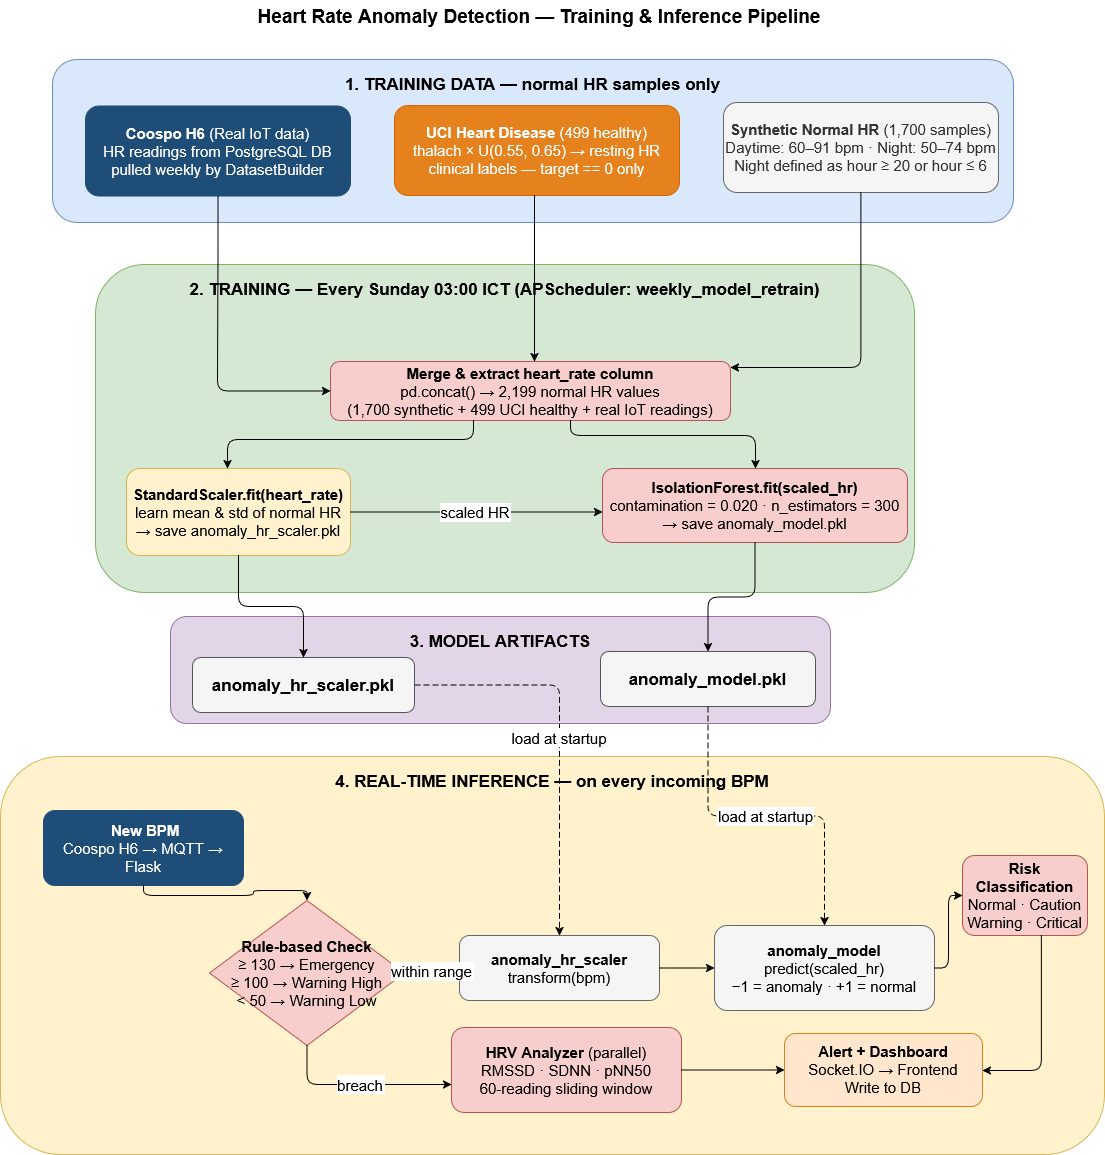
\includegraphics[width=\textwidth]{images/fig_hr_anomaly_pipeline.png}
\caption[Heart rate anomaly detection pipeline: training and inference]{%
         Heart rate anomaly detection pipeline.
         \textbf{Training} (top, repeated every Sunday at 03:00 by
         \texttt{weekly\_model\_retrain}): normal HR samples from three
         sources — real IoT readings (Coospo H6), 499 UCI Heart Disease
         healthy records converted from \textit{thalach}, and 1\,700
         synthetic day/night samples — are merged, scaled with a
         dedicated \texttt{StandardScaler}, and used to fit an
         \texttt{IsolationForest} (\texttt{contamination}=0.020,
         \texttt{n\_estimators}=300).
         \textbf{Inference} (bottom, per incoming BPM): each reading
         passes a rule-based threshold check first; readings within range
         are forwarded to the scaler then the model for anomaly scoring
         and risk classification.}
\label{fig:ml_pipeline}
\end{figure}

\FloatBarrier

\paragraph{Periodic Model Retraining}
\label{subsec:periodic_retrain}

Two separate training scripts serve distinct roles in this system.
\texttt{tune\_and\_retrain\_anomaly.py} is a standalone offline script
that produced the initial model and all evaluation metrics reported in
Chapter~\ref{chap:experiments} (Table~\ref{tab:feature_ablation}); it
operates without database access and trains exclusively on the
UCI~+~synthetic baseline (2\,199 samples).
\texttt{train\_pipeline.py}, by contrast, is the live backend pipeline
invoked by the scheduler: it pulls accumulated sensor readings directly
from the database, merges them with the UCI baseline and a shrinking
synthetic buffer, and overwrites the deployed model artefacts in place.
The two scripts share the same contamination value (0.020) and model
architecture but differ in data composition as real IoT readings build up
over time.

The Isolation Forest and the three companion models (automation classifier,
mood classifier, shared scaler) are retrained automatically every Sunday
at 03:00~(Asia/Ho\_Chi\_Minh) by an APScheduler \texttt{BackgroundScheduler}
job registered at server startup (\texttt{weekly\_model\_retrain}).
The job calls \texttt{run\_full\_training()} inside a Flask application
context so that \texttt{DatasetBuilder} can access the database.

Each retrain pass merges three data sources into a shared DataFrame:
\begin{enumerate}
    \item \textbf{Real IoT sensor data} (from the \texttt{sensor\_data} table) ---
    accumulated readings from the deployed ESP32 node and Coospo~H6 device,
    resampled at 5-minute intervals.
    \item \textbf{UCI Heart Disease healthy records} (499 rows, \texttt{target}~=~0)
    --- a fixed clinical baseline loaded from \texttt{data/heart\_disease.csv}.
    \item \textbf{Synthetic normal samples} --- the count decreases automatically
    as real IoT data grows, following the five-stage dilution schedule in
    Table~\ref{tab:dilution}.
\end{enumerate}

The four models trained from this DataFrame use different feature subsets.
The \textbf{anomaly model} extracts only the \texttt{heart\_rate} column and
fits a dedicated HR scaler (\texttt{anomaly\_hr\_scaler.pkl}), keeping
\texttt{contamination}~=~0.020 as established by grid search.
Room context features (temperature, humidity, light) are excluded because
they dilute the cardiac signal: each Isolation Forest tree samples uniformly
from all features, so adding six context columns reduces the probability of
selecting \texttt{heart\_rate} to 1-in-7~\cite{Liu2008}.
The \textbf{automation} and \textbf{physiological state (mood)} classifiers
use the full 7-feature scaled matrix; their design and label sources are
described in Section~\ref{sec:companion_classifiers}.

\begin{table}[H]
\centering
\caption[Synthetic dilution schedule]{Synthetic dilution schedule in \texttt{\_choose\_synthetic\_samples()}}
\label{tab:dilution}
\small
\begin{tabular}{@{} l r l @{}}
\toprule
\textbf{Stage} & \textbf{Synthetic samples added} & \textbf{Rationale} \\
\midrule
$<$10 real rows       & 1\,700 & Cold-start bootstrap \\
10--599 real rows     & 1\,700 & UCI-seed phase (matching baseline) \\
600--999 real rows    & $\max(300,\ \lfloor\text{real}{\times}0.50\rfloor)$ & Growth phase \\
1\,000--4\,999 real rows & $\max(40,\ \lfloor\text{real}{\times}0.20\rfloor)$ & Mature phase \\
$\geq$5\,000 real rows   & 0 & Real-dominant, no synthetic needed \\
\bottomrule
\end{tabular}
\end{table}

As deployment time increases, the model progressively shifts from
synthetic-dominant to real-data-dominant training, improving its fit
to the specific user's circadian HR patterns.
Job failures are caught and logged at \texttt{ERROR} level; they do not
propagate to the scheduler thread, so a failed retrain does not affect
the running inference pipeline.

% ─────────────────────────────────────────────────────────────
\subsection{Companion Classifiers: Physiological State and Automation}
\label{sec:companion_classifiers}

The training pipeline produces two RandomForest classifiers alongside the
anomaly model.  They share the same 7-feature scaled matrix and are retrained
weekly, but serve entirely different purposes from the anomaly detector.

\paragraph{Physiological State (Mood) Classifier}

The physiological state classifier assigns each incoming BPM reading one of
seven context-aware labels: \texttt{EMERGENCY}, \texttt{ELEVATED},
\texttt{QUIET}, \texttt{SLEEP}, \texttt{REST}, \texttt{ACTIVE}, or
\texttt{NORMAL}.  Because no labelled dataset of real physiological states
with time-stamped sensor readings exists, the training labels are generated
by a deterministic rule function (\texttt{\_calc\_mood}) that maps sensor
values to states using published elderly HR norms and circadian patterns:

\begin{itemize}
    \item \textbf{EMERGENCY}: HR~$\geq130$\,bpm (checked first — unconditional)
    \item \textbf{ELEVATED}: HR~$\geq100$\,bpm
    \item \textbf{QUIET}: night-time ($\text{is\_night}=1$) and light\_level~$<20$ (0--100 scale)
    \item \textbf{SLEEP}: night-time and HR~$<65$\,bpm
    \item \textbf{REST}: HR~$<60$\,bpm with elevated room temperature ($>28\,^\circ$C)
    \item \textbf{ACTIVE}: HR~$\geq80$\,bpm with high ambient light (light\_level~$>60$, 0--100 scale)
    \item \textbf{NORMAL}: all other readings — none of the above conditions met (fallback label)
\end{itemize}

Rather than applying the rules as a direct lookup, a RandomForest is trained on pseudo-labels produced by \texttt{\_calc\_mood} to handle readings that fall between hard thresholds --- the model inherits the label semantics of the rules but uses the surrounding training distribution to assign a class rather than forcing a binary condition check. It cannot discover categories beyond what the rules define, and its boundary behaviour has not been validated against ground-truth physiological annotations (see evaluation note below).
The predicted state is attached to each \texttt{hr\_alert} Socket.IO event, stored in \texttt{patient\_hr\_record}, and exported in health report PDFs in the ``RISK\,/\,MOOD'' column.

The automation classifier is trained using real user behaviour: labels (\texttt{action\_label}) derived from the \texttt{ControlLog} table, matched with sensor readings in the 2-minute window prior to the device action. 
The model can improve as the household accumulates usage data through weekly retraining. \textbf{Evaluation note.} Neither classifier has been independently and quantitatively evaluated. The mood classifier labels are purely determined by \texttt{\_calc\_mood}. Boundary smoothing by RandomForest cannot be validated without ground-truth annotations. The automation classifier does not have enough logged events at the prototype stage to measure meaningful precision/recall. A quantitative evaluation of both is left for future work (Section~\ref{sec:future}).

% ─────────────────────────────────────────────────────────────
\subsection{Alfred AI Assistant}
\label{sec:alfred_method}

Alfred is a conversational assistant for health monitoring and smart home control. It runs in one of three inference modes, selectable per request:
\begin{itemize}
\item \textbf{llm} (default): The full 3-layer pipeline. The message goes through the deterministic Rule layer (device control, mood detection, keyword matching) first. If no match is found, it falls back to an Ollama \texttt{qwen2.5:3b} intent parser. If no intent is found, it is passed to a context-enriched Ollama chat call.

\item \textbf{rule}: Uses only deterministic keyword and pattern matching. It runs entirely offline with minimal latency and provides a clarification fallback when no rule matches.

\item \textbf{gemini}: Sends the context-enriched prompt to Google Gemini~2.5~Flash via the \texttt{google-genai} SDK. If the cloud service is unavailable, a Rule engine fallback response is returned rather than switching inference paths.

\end{itemize}

A frontend \textbf{Compare} overlay calls \texttt{rule}, \texttt{llm}, and
\texttt{gemini} modes sequentially and presents the three responses
side-by-side. Before each inference call, the backend injects live device
states and sensor readings into the prompt, ensuring Alfred always has access
to current home state without a retrieval-augmented architecture.

\paragraph{Context injection versus retrieval-augmented generation.}
\label{par:context_vs_rag}
A conventional RAG pipeline retrieves document chunks from a vector store before generating a response. That design is well-suited to large, slowly changing knowledge bases --- medical literature, product manuals, FAQ corpora --- where the information is too voluminous to fit in a prompt and is updated infrequently enough that a slightly stale retrieval result is acceptable. Alfred operates over a fundamentally different kind of data. The house context --- room names, relay states, sensor readings --- is small enough to serialize into a short prompt prefix, is authoritative at request time because it is read directly from the live database, and changes fast enough that a cached embedding in a vector store would be stale within seconds of a relay toggle. Under these conditions, direct injection is not a simplification of RAG; it is the appropriate design choice. A retrieval step would add embedding-query latency and introduce the risk of serving outdated state without providing any benefit that is not already met by a direct database read.

The practical limit of this approach is context window size. At the current prototype scale --- one ESP32 node, up to eight sensors, and two to five devices per room --- the serialized house prefix fits comfortably within 100 tokens, well inside the limits of both \texttt{qwen2.5:3b} and Gemini~2.5~Flash. If the deployment were extended to dozens of rooms and hundreds of devices, selective injection (e.g., filtering to the user's active room before prompt construction) would be necessary. That path is noted as a Phase~2 architectural consideration in Section~\ref{sec:future}.

\paragraph{Local LLM Selection Rationale}
\label{subsec:llm_selection}

\texttt{qwen2.5:3b} (Q4\_K\_M, $\approx$2\,GB) was selected for local inference for three reasons: (1) it runs comfortably on the 16\,GB development machine alongside the Flask backend and MySQL process; (2) it supports Vietnamese and English without translation, enabling mixed-language input; and (3) preliminary tests showed that it follows the desired JSON schema (\texttt{\{action, target\_device, value, reply\}}) more reliably than the alternatives tested (\texttt{gemma2:2b}, \texttt{phi3.5-mini}). A formal, multi-model comparison is deferred to future work (Section~\ref{sec:future}).

\paragraph{Mode-wise Request Processing}

The REST endpoint is the same for all chat modes: \path{POST /api/ai/chat}, with the same fields: \path{message}, \path{mode} and \path{language}. The difference is that \path{AIUseCase.handle\_chat()} interprets the message against the real-time house context that was loaded. Table~\ref{tab:alfred_mode_behavior} illustrates the different handling of the same utterance across the three modes.

\begin{table}[H]
\centering
\caption[Alfred utterance handling across modes]{How the same utterance is handled across Alfred modes}
\label{tab:alfred_mode_behavior}
\small
\begin{tabularx}{\textwidth}{@{} l >{\hsize=0.55\hsize\RaggedRight\arraybackslash}X >{\hsize=1.45\hsize\RaggedRight\arraybackslash}X @{}}
\toprule
\textbf{Mode} & \textbf{Backend path} & \textbf{Example behavior for ``nóng quá''} \\
\midrule
LLM        & Rule $\to$ Intent Parser $\to$ Ollama chat
           & Environmental keyword ``nóng'' matched by Rule layer; fan and AC scenario suggested with a confirmation prompt. If Rule did not match, Intent Parser would parse intent; Chat LLM handles open-ended fallback. \\
\addlinespace[4pt]
Rule       & Rule engine only (keyword/pattern)
           & ``nóng'' matches the \textit{hot} environmental intent; returns a device suggestion with confirmation prompt. If unmatched, returns clarification fallback --- no LLM call made. \\
\addlinespace[4pt]
Gemini     & Rule $\to$ Gemini 2.5 Flash (cloud)
           & Rule layer runs first --- ``nóng'' is caught and a confirmation prompt returned, same as Rule mode. If Rule misses, the context-enriched prompt goes to Gemini Flash. API unavailability falls back to the Rule clarification reply. \\
\bottomrule
\end{tabularx}
\end{table}

In short, there is no separate frontend endpoint per mode, mode selection changes backend reasoning strategy, not the transport path. Table~\ref{tab:alfred_layer_matrix} summarises which layers are activated in each mode.

\begin{table}[H]
\centering
\caption{Layer activation per Alfred inference mode}
\label{tab:alfred_layer_matrix}
\small
\begin{tabularx}{\textwidth}{@{}l X X X@{}}
\toprule
\textbf{Mode} & \makecell[l]{\textbf{Layer 1 —}\\\textbf{Rule Engine}} & \makecell[l]{\textbf{Layer 2 —}\\\textbf{Intent Parser}} & \makecell[l]{\textbf{Layer 3 —}\\\textbf{Chat LLM}} \\
\midrule
\texttt{llm}    & \checkmark\ keyword/pattern match & \checkmark\ Ollama (if Rule misses)  & \checkmark\ Ollama (if Intent misses) \\
\texttt{rule}   & \checkmark\ keyword/pattern match & \texttimes\ stops here               & \texttimes\ not called \\
\texttt{gemini} & \checkmark\ keyword/pattern match & \texttimes\ bypassed$^\dagger$        & \checkmark\ Gemini Flash \\
\bottomrule
\end{tabularx}
\smallskip\noindent{\footnotesize$^\dagger$ Gemini Flash handles intent classification and response generation in a single cloud call, so there is no need for a separate intent-parser step.}
\end{table}

\paragraph{Layer design rationale.}
The three-layer LLM pipeline assigns each layer a distinct role matched to its cost and latency profile:

\begin{itemize}
    \item \textbf{Layer~1 (Rule)} handles the majority of everyday commands --- device on/off, mood detection, room queries --- with deterministic keyword matching at negligible latency and zero API cost. It is always executed first in LLM and Gemini modes because it covers the most common intents cheaply.

    \item \textbf{Layer~2 (Intent Parser)} is a lightweight Ollama call ($\approx$100-token prompt) whose sole job is to classify an unmatched message into a fixed schema \texttt{\{intent, action, device\_type, room\}}. Rule is not reused here because if a message did not match Layer~1 it will not match again; Gemini is not used because a structured classification task does not justify cloud API latency or cost.

    \item \textbf{Layer~3 (Chat LLM)} generates the final natural-language response with full house-context injection. Gemini mode skips Layer~2 entirely and calls Gemini once for both intent and response, since Gemini can handle both classification and generation in one call.
\end{itemize}


Every incoming message runs through a nine-step early-exit waterfall in \texttt{AIUseCase.handle\_chat()}. The steps are checked in order, and the first one to match wins: as soon as a step handles the message and returns, nothing below it executes.

\textbf{Step~1} (SOS) outranks everything else. A distress keyword fires a critical alert, emails the caregiver, and returns before any other logic gets a look in. \textbf{Step~2} (FAQ) answers predictable platform questions from a hardcoded table, and only in rule mode, so the system never spends an LLM call on them. \textbf{Step~3} (Pending) clears a queued yes/no confirmation, either running the stored MQTT command or dropping it. \textbf{Step~4} (Schedule) reacts to a time or recurrence cue, parsing the cron expression through \texttt{\_apply\_daypart()} and asking for a specific clock time when the hour is ambiguous.

\textbf{Step~5} (Info query) pulls sensor, health, or device-status answers straight from the live house-context object and sends no MQTT command at all. \textbf{Step~6} (Device control) identifies target devices with word-boundary regular expressions, resolves the room, and stores a pending confirmation before it publishes anything. That two-step guard is deliberate: a stray keyword match should never flip a relay on its own. \textbf{Steps~7--8} (Small-talk and Mood) field greetings and read mood keywords to suggest a lighting or climate change, again pausing for confirmation whenever a real device would be touched.

\textbf{Step~9} (Fallback) is the only step whose behaviour depends on the mode. In \texttt{rule} mode it just returns a clarification prompt and calls no model. In \texttt{gemini} mode it forwards a context-enriched prompt to Gemini~2.5~Flash. In \texttt{llm} mode it calls \texttt{parse\_intent()} for a structured \texttt{\{intent, action, device\_type, room\}} classification, then branches on the result: \textit{control} resolves devices and stores a confirmation, \textit{query} answers from live context, \textit{chat} returns the model's reply, and \textit{add}/\textit{delete} run device-registry CRUD.

\paragraph{Alfred End-to-End Processing Flow}
\label{subsec:alfred_e2e_flow}

\texttt{AIUseCase.handle\_chat()} first loads a live house-context object (rooms, device relay states, latest sensor readings), cached per user with a 10-second TTL. When passed to an LLM, this context is serialized into a compact prompt prefix (e.g., \texttt{"Living Room: den\_1 (ON), quat\_1 (OFF)"}) to ground the model in the current home state without overflowing the context window. What happens next depends on the selected mode:

\begin{itemize}
   \item \textbf{LLM mode} runs the complete three-layer pipeline via the local Ollama backend. The message hits the deterministic Rule layer first (keyword matching, device control, mood and scenario detection). If nothing matches, a lightweight Ollama intent-parser call (\textasciitilde{}100-token prompt) classifies the intent as \texttt{control}, \texttt{query}, or \texttt{chat}. Anything still unresolved falls through to a context-enriched Ollama chat call where the full house structure and device codes are injected into the prompt.

\item \textbf{Rule mode} executes only the Rule layer and returns a clarification fallback if nothing matches --- no LLM call is made.

\item \textbf{Gemini mode} first executes the Rule layer and if unmatched, forwards the context-enriched prompt to Google Gemini~2.5~Flash. If the Gemini API is unavailable, the mode returns the Rule engine's clarification fallback rather than switching to the Ollama path.

\end{itemize}

\paragraph{Real-time device resolution.} \texttt{alfred\_knowledge.py} only stores device categories (e.g., \texttt{"ac"}, \texttt{"fan"}), not specific identifiers. If a rule matches, \texttt{AIUseCase} resolves the category to physical devices with \texttt{\_find\_devices\_by\_category()}, filtered by the room the user is currently in (set by double-clicking a room on the floor plan). If there is no such device, the action is skipped. If there are devices in more than one room, the backend asks the user to select.

\paragraph{Two-step confirmation.}
Alfred \emph{does not} execute immediately when it recognizes a device action. Instead, it stores a \texttt{pending\_action} and responds with a confirmation prompt. If the answer is affirmative (\textit{có}, \textit{yes}, \textit{đồng ý}), it calls \texttt{DeviceUseCase.set\_device()}, which publishes the MQTT command (TLS port~8883) and broadcasts the new state via Socket.IO. The pending action times out after 90 seconds. Only scheduled automation rules can run automatically without confirmation.

\paragraph{Multi-room disambiguation}
A related case arises when a matched scenario involves devices spread across several rooms. Alfred cannot safely assume which room to act on, so it asks the user to specify. The narrowed plan is held in \texttt{pending\_action} and a second confirmation is required before anything runs. One shortcut exists: if the user has already indicated their current location by double-clicking a room on the floor plan, the system filters the plan down to that room and skips straight to the confirmation step. Even so, the command is never sent without a reply from the user.

\paragraph{Rule Engine Keyword and Intent Taxonomy} \label{sec:alfred_rule_keywords}

Keyword matching in \texttt{alfred\_knowledge.py} is organised into three groups, evaluated by the Rule engine using case-insensitive substring search:

\begin{itemize}
    \item \textbf{Mood Profiles} (\texttt{MOOD\_PROFILES}) --- eight emotional states, ranging from happy and excited to sick and stressed, each paired with lighting adjustments, climate presets, and optional music or film suggestions.

    \item \textbf{Environmental Intents} (\texttt{ENVIRONMENTAL\_INTENTS}) --- four physical-condition triggers (\textit{hot}, \textit{cold}, \textit{dark}, \textit{bright}) that map directly to device actions. Rather than referencing specific device names, each entry targets a \texttt{category} value (e.g. \texttt{"fan"}, \texttt{"ac"}, \texttt{"light"}) that the system resolves to the actual installed device at query time. This means adding a new fan or replacing a light requires no change to the intent definitions. As a concrete example, saying ``too hot'' activates the \textit{hot} intent: the fan turns on at speed~3 and the air conditioner is set to 24\,°C.

    \item \textbf{Device Scenarios} (\texttt{ALFRED\_SCENARIOS}) --- eleven activity-based presets covering common routines such as going to sleep, studying, watching a film, or leaving the house. The four environmental entries in this dictionary point back to \texttt{ENVIRONMENTAL\_INTENTS} rather than repeating the definitions, so adjusting a default --- the fan speed when it feels too hot, for example --- only ever needs changing in one place.
\end{itemize}

The taxonomy covers around 20 intent categories and roughly 200 Vietnamese--English keyword triggers in total (see Appendix~\ref{app:alfred_keywords}, Table~\ref{tab:alfred_rule_keywords}). Scenarios and environmental intents are checked first; mood profiles follow. If nothing matches, the message moves on to the LLM step.

\paragraph{Natural Language Device Scheduling}

Before the LLM step, Alfred also checks whether the user is trying to set up a recurring device schedule. A dedicated \texttt{schedule\_intent\_parser} scans the message for a device reference, a clock time, and a recurrence pattern using a set of Vietnamese--English regex rules. Recognised patterns include \textit{daily}, \textit{weekday}, \textit{weekend}, and \textit{specific days of week}: for example, ``turn off the fan on Monday and Thursday at 9 pm'' is parsed into the cron expression \texttt{0 21 * * 1,4} and written to the \texttt{schedules} table. Day names in both languages are matched with word-boundary guards so that ``thu'' in ``thursday'' does not accidentally match the Vietnamese abbreviation ``T5.'' If only some components are present (e.g.\ a day name but no device), Alfred asks a follow-up question rather than guessing. Confirmed schedules are visible on the Care~\&~Schedule page and can be edited or deleted from there.

% ─────────────────────────────────────────────────────────────
\section{System Interaction Design}
\label{sec:seq_method}

Two sequence diagrams illustrate the critical runtime data flows.
Figure~\ref{fig:seq_device_method} shows the end-to-end path of a
user-initiated device toggle command from the web dashboard through the
Flask REST API and EMQX broker to the ESP32 relay, and back as a Socket.IO
confirmation event. Figure~\ref{fig:seq_health_method} shows the anomaly
detection path from a BLE heart-rate reading through to a real-time
client alert.

\begin{landscape}
\begin{figure}[p]
\centering
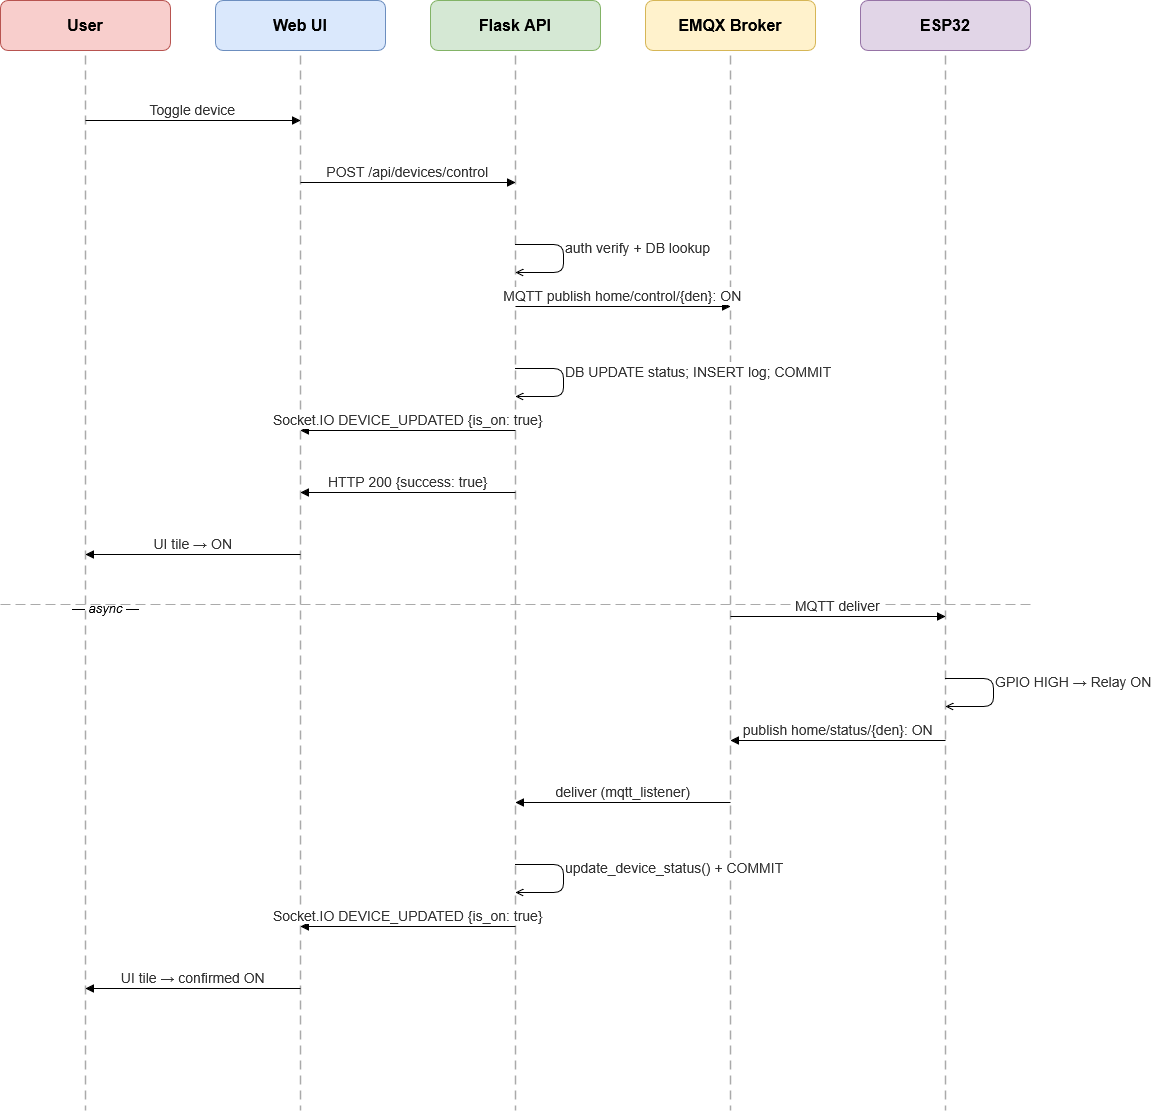
\includegraphics[width=\linewidth,height=0.80\textwidth,keepaspectratio]{images/fig_seq_s1.png}
\caption[Sequence S1: device control flow]{Sequence S1: end-to-end device control flow from web dashboard to ESP32 relay and back via Socket.IO.}
\label{fig:seq_device_method}
\end{figure}
\end{landscape}

\begin{landscape}
\begin{figure}[p]
\centering
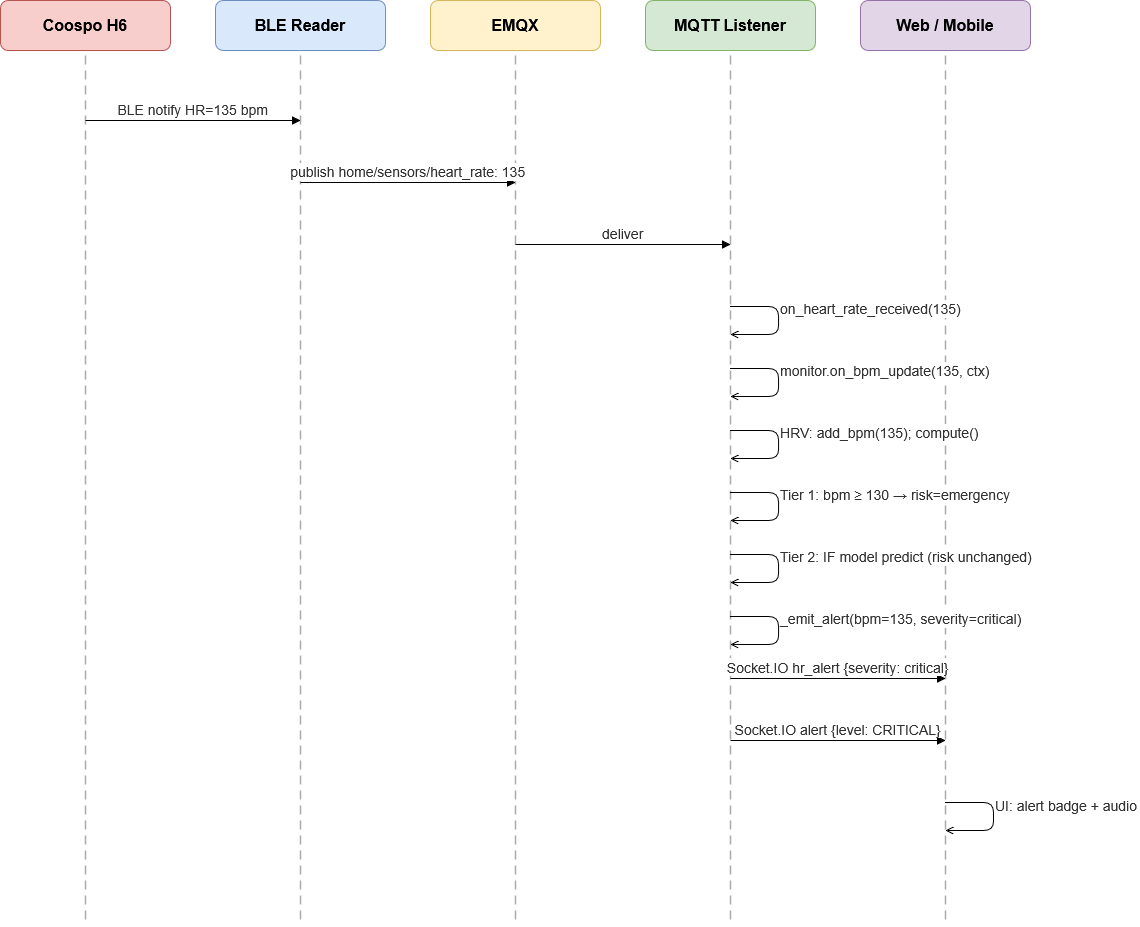
\includegraphics[width=\linewidth,height=0.80\textwidth,keepaspectratio]{images/fig_seq_s2.png}
\caption[Sequence S2: BLE heart-rate alert flow]{Sequence S2: BLE heart-rate reading to critical alert propagation across all system layers.}
\label{fig:seq_health_method}
\end{figure}
\end{landscape}


